\documentclass[10pt]{article}
\usepackage[letterpaper, margin=1in]{geometry}
\usepackage[T1]{fontenc}
\usepackage{lmodern}
\usepackage[utf8]{inputenc}
\usepackage{microtype}
\usepackage{amsmath, amssymb}
\usepackage{booktabs, tabularx, multirow, array}
\usepackage{graphicx}
\usepackage{xcolor}
\usepackage{enumitem}
\usepackage{fancyvrb}
\usepackage{caption}
\usepackage[numbers, sort&compress]{natbib}
\usepackage{tikz}
\usetikzlibrary{positioning,arrows.meta,fit,backgrounds,shapes.geometric,calc,shapes.misc}
\definecolor{semblue}{HTML}{2A78D6}
\definecolor{semorange}{HTML}{EB6834}
\definecolor{ink}{HTML}{222222}
\definecolor{inkmuted}{HTML}{666666}

\usepackage[colorlinks=true, linkcolor=semblue, citecolor=semblue, urlcolor=semblue]{hyperref}
% generated by scripts/make_figures_tables.py from the released result JSONs -- do not edit
\newcommand{\eepDev}{29/30}
\newcommand{\eepLocked}{20/20}
\newcommand{\pdLocked}{20/20}
\newcommand{\pdFalseAccept}{0}
\newcommand{\pdLlmOnly}{0}
\newcommand{\pdDiscoveries}{32}
\newcommand{\nlScenario}{.867}
\newcommand{\nlLearned}{.914}
\newcommand{\nlWrongExec}{1}
\newcommand{\nlWrongProposed}{22}
\newcommand{\nlWrongBlocked}{16}
\newcommand{\nlFalseAccept}{1}
\newcommand{\nlDirect}{5.6}
\newcommand{\nlTrace}{86.1}
\newcommand{\pdxTeacherLearned}{24/36}
\newcommand{\pdxScriptedLearned}{33/36}
\newcommand{\pdxWrong}{12}
\newcommand{\pdxFalseAccept}{1}
\newcommand{\pdxRetention}{54/54}
\newcommand{\htgDLearned}{27/36}
\newcommand{\htgDGround}{1.0}
\newcommand{\htgDWrong}{2}
\newcommand{\ttpDLearned}{31/36}
\newcommand{\ttpDWrong}{0}
\newcommand{\rciDLearnedPooled}{70/72}
\newcommand{\rciDLearnedPooledFrac}{.972}
\newcommand{\rciDLearnedA}{36/36}
\newcommand{\rciDLearnedB}{34/36}
\newcommand{\rciDLearnedMin}{65}
\newcommand{\rciDScenarioPooled}{58/60}
\newcommand{\rciDScenarioPooledFrac}{.967}
\newcommand{\rciDScenarioA}{30/30}
\newcommand{\rciDScenarioB}{28/30}
\newcommand{\rciDScenarioMin}{54}
\newcommand{\rciDDistilledPooled}{62/64}
\newcommand{\rciDDistilledPooledFrac}{.969}
\newcommand{\rciDDistilledA}{32/32}
\newcommand{\rciDDistilledB}{30/32}
\newcommand{\rciDDistilledMin}{58}
\newcommand{\rciDGroundingPooled}{71/71}
\newcommand{\rciDGroundingPooledFrac}{1.0}
\newcommand{\rciDGroundingA}{36/36}
\newcommand{\rciDGroundingB}{35/35}
\newcommand{\rciDGroundingMin}{68}
\newcommand{\rciCeiling}{4/5}
\newcommand{\rciFingerprint}{dacd7a90}
\newcommand{\rciSpend}{3.57}
\newcommand{\lockedLearned}{23/23}
\newcommand{\lockedScenario}{20/20}
\newcommand{\lockedDistilled}{21/21}
\newcommand{\lockedGround}{22/23}
\newcommand{\lockedGroundFrac}{.957}
\newcommand{\sfifteenTests}{20/20}


\captionsetup{font=small, labelfont=bf}
\setlist{itemsep=1pt, topsep=3pt}
\makeatletter\g@addto@macro\UrlBreaks{\do\_\do\-\do\:\do\.}\makeatother
\Urlmuskip=0mu plus 1mu
\newcommand{\id}[1]{\nolinkurl{#1}}
\newcommand{\semvm}{SEMVM}
\newcommand{\lockedsentence}{The sealed LOCKED evaluation passed every behavioral acquisition, grounding, safety, and reuse criterion, but failed the preregistered proof-of-teacher-disconnection condition because teardown was probed before the hosted endpoint had fully disappeared.}
\fvset{fontsize=\scriptsize, frame=single, framesep=2mm, rulecolor=\color{black!30}}

\title{\textbf{External Procedural Distillation:\\ Natural-Language Teaching into Verified Procedural Memory with a Frozen Student}}
\author{Matthew Anderson\\ \small\texttt{github.com/sheriffoftiltover/stateful-semantic-vm}}
\date{September 2026 \quad (preprint; not peer reviewed)}

\begin{document}
\maketitle

\begin{abstract}
\noindent
We study whether a system built around a small, frozen language model can acquire new procedural capability from a larger model without any change to its own neural weights. In the Stateful Semantic Virtual Machine (\semvm), neural models only propose and never hold state: the world lives in a SQLite store that models reach only through typed queries, and durable state, execution, and every learning decision are deterministic. A hosted teacher (gpt-oss-120b) teaches a skill in natural language. A transactional teaching controller has each lesson line grounded into a typed plan (by a hosted grounder), executes it inside a sandboxed SQLite world, and admits a demonstration as evidence only if it is complete and committed. A deterministic anti-unifier proposes a parameterized program, and an evidence verifier (replay, counterfactual argument substitution, state perturbation, negative cases, rollback injection, determinism) decides whether it may be activated in a persistent procedure library. The hosted models are then destroyed, and the skill is used from fresh processes under a network guard, with a frozen Qwen2.5-Coder-1.5B model interpreting requests behind deterministic checks.
We report a seven-experiment preregistered lineage in a synthetic, bounded personal-organizer domain. In the final experiment, two resource changes---a teacher example-value pool of 4 instead of 2 and a teacher output budget of 8{,}192 instead of 4{,}096 tokens---raised the hosted-teacher/hosted-grounder arm to \rciDLearnedPooled\ exactly learned procedures pooled over two independent development draws (\rciDLearnedA\ and \rciDLearnedB), with zero wrong committed actions; the parent experiment had \ttpDLearned\ on its own draw.
\lockedsentence\ Behaviorally, LOCKED produced \lockedLearned\ exactly learned procedures and \lockedScenario\ exact scenarios, with zero post-handoff hosted calls or network attempts; it is nonetheless not a clean pass. The results support a narrow claim: \semvm\ can accumulate externally stored, verified procedural capability acquired with assistance from a temporary teacher. The teacher is in the acquisition causal chain, not the execution causal chain, and continued growth of the library currently depends on access to a teacher or other source of usable demonstrations.
\end{abstract}

\section{Introduction}\label{sec:intro}

A deployed model that must learn new, reusable behaviors faces a familiar trade-off. Updating its weights risks interference with what it already does \citep{mccloskey1989catastrophic, kirkpatrick2017ewc}; distilling from a larger model transfers behavior through training data or soft targets \citep{hinton2015distilling, kim2016sequence, hsieh2023distilling} but requires a training run, and the transferred behavior is not individually inspectable. A third option is to keep the model frozen and put the learned capability somewhere else.

This paper describes one concrete version of that option and the preregistered experiments that shaped it. In \semvm\ (Stateful Semantic Virtual Machine), a learned skill is a small typed program stored in a SQLite procedure library, with its source evidence, version history and verification record. The program is not written by a language model. It is abstracted by a deterministic anti-unifier from traces that the system itself executed while a teacher demonstrated the skill in natural language, and it becomes executable only after a deterministic verifier has tested it against that evidence. The student's neural weights never change; their byte-level hash is checked in every process.

We use the term \emph{external procedural distillation} for this setting: a capability demonstrated by a larger model ends up as verified external memory of a smaller system. The term is deliberately narrow. The 1.5B model does not learn the 120B model's knowledge; no weights are trained; nothing is distilled into parameters. What is transferred is a procedure, and what makes it trustworthy is not the teacher's authority but the evidence and the verifier.

\paragraph{Core claim.} The \semvm\ system can accumulate externally stored procedural capability, acquired with assistance from a temporary teacher, without modifying the frozen student's neural weights. Continued growth of that library currently depends on access to a teacher or other source capable of supplying usable demonstrations. The teacher sits in the \emph{acquisition} causal chain; after handoff it is absent from the \emph{execution} causal chain (Figure~\ref{fig:handoff}).

\paragraph{What we do not claim.} We do not claim that the 1.5B model learned the 120B model's knowledge; classical (weight-level) distillation; open-domain continual learning; autonomous self-improvement; arbitrary program synthesis; indefinite scaling of the library; or human-level generality. We do not claim that the final LOCKED evaluation was a formally clean pass: it was not (Section~\ref{sec:locked}).

\paragraph{Contributions.}
\begin{enumerate}
\item An architecture in which neural components (teacher, grounder, request interpreter) have proposal authority only and never hold state: the world is read through typed queries executed by a deterministic runtime, which holds all decision authority over state, evidence admission and procedure activation (Section~\ref{sec:system}, Tables~\ref{tab:components} and~\ref{tab:monolithic}).
\item A transactional teaching protocol: a demonstration is a sandboxed transaction over a slot ledger that either commits complete evidence or aborts with zero evidence (Figure~\ref{fig:lifecycle}).
\item A preregistered lineage of seven experiments, including negative and invalid runs, that locates the bottleneck step by step: runtime, procedure induction, natural-language grounding, teacher channel, clarification protocol, transactional safety, and finally recovery capacity (Section~\ref{sec:lineage}, Figure~\ref{fig:progression}).
\item A $2\times2$ factorial over lesson source and recovery source, replicated on two independent development draws, showing that once resources suffice these factors move acquisition by at most a few targets and in inconsistent directions (Section~\ref{sec:rci}).
\item A fully disclosed LOCKED result whose behavioral criteria all pass but whose preregistered teardown-proof condition fails, reported as such (Section~\ref{sec:locked}), and a released artifact bundle with raw teacher, grounder and verifier records (Section~\ref{sec:repro}).
\end{enumerate}

\section{Related work}\label{sec:related}

\paragraph{Knowledge distillation and continual learning.} Distillation transfers a teacher's behavior into student weights through soft targets \citep{hinton2015distilling}, sequence-level outputs \citep{kim2016sequence} or rationales \citep{hsieh2023distilling}. Continual learning studies how to add capability to weights without catastrophic interference \citep{mccloskey1989catastrophic, kirkpatrick2017ewc}. \semvm\ sidesteps both by never training the student: the transferred object is an external program, so interference with existing weights cannot occur, but neither does the student's general competence improve.

\paragraph{Retrieval and external memory.} Retrieval-augmented generation conditions a model on retrieved text \citep{lewis2020rag}; memory-management systems page information in and out of a context window \citep{packer2023memgpt}; differentiable memories make storage part of the network \citep{graves2014ntm}. In these systems the retrieved content is read by the model and influences generation. In \semvm\ the stored object is executed by a deterministic VM; the language model at reuse time only ranks candidate procedure names and writes an argument list, both of which are checked (Section~\ref{sec:system}). A wrong retrieval can cause a clarification or an incorrect choice of procedure, but it cannot alter what a stored procedure does.

\paragraph{Tool making and skill libraries for LLM agents.} LLMs can write reusable tools \citep{cai2024latm, yuan2024craft}, accumulate skill code in open-ended environments \citep{wang2023voyager}, induce reusable workflows from experience \citep{wang2024awm}, or store textual insights \citep{zhao2024expel, shinn2023reflexion}; tool-use models call APIs \citep{schick2023toolformer, patil2024gorilla, yao2023react}, and program-aided models offload computation to an interpreter \citep{gao2023pal}. These systems typically let the LLM author the stored artifact and validate it by task success or execution feedback. \semvm\ differs in where authority sits: the stored program is derived from executed, committed traces by a deterministic abstraction step, and its activation is decided by evidence tests that include counterfactual and perturbation checks designed to catch programs that are consistent with the demonstrations yet wrong (Section~\ref{sec:verifier}). In our own lineage, the 1.5B model's direct program proposals added nothing over anti-unification (Section~\ref{sec:lineage}).

\paragraph{Library learning and program induction.} DreamCoder \citep{ellis2021dreamcoder} and LILO \citep{grand2024lilo} compress solved programs into reusable abstractions; \citet{berlotattwell2024library} caution that measured gains in LLM library learning can come from other factors than reuse. Our abstraction step is anti-unification-style generalization \citep{plotkin1970note} over a small typed step language, closer in spirit to programming-by-example systems such as FlashFill \citep{gulwani2011flashfill}. We make no claim about library-learning at scale; our reuse measurements are direct (the stored procedure is invoked after restarts with new arguments and wording).

\paragraph{Learning procedures from instruction and demonstration.} Programming by demonstration \citep{cypher1993watch}, instructable agents that learn procedures from natural-language dialogue \citep{azaria2016lia}, multimodal demonstration systems \citep{li2017sugilite} and collaborative task learning from a single session of demonstration and dialogue \citep{allen2007plow} are the closest ancestors of the teaching setting. Our teacher is a model rather than a person, the student is a frozen small model plus a deterministic runtime, and the protocol is evaluated with preregistered gates and sealed test sets.

\paragraph{Semantic parsing and neural program execution.} Grounding language into executable forms is classical semantic parsing \citep{zettlemoyer2005learning, liang2011dcs}; dataflow dialogue \citep{andreas2020dataflow} is a close relative of our reference handling. Neural program interpreters \citep{reed2016npi} learn to execute programs in weights, whereas \semvm\ keeps execution symbolic. Compositional generalization failures of sequence models \citep{lake2018scan} motivated our earlier choice to place state and bookkeeping outside the network.

\section{System}\label{sec:system}

\subsection{Overview and authority boundaries}

Figure~\ref{fig:arch} shows the final configuration and Table~\ref{tab:components} lists each component with what it may and may not do. The organizing rule is that neural components produce \emph{proposals} (lesson text, a typed plan for one line, a ranking of procedure names, an argument string), and deterministic components decide whether anything is executed, admitted as evidence, or activated.

\begin{figure}[t]
\centering
\resizebox{\linewidth}{!}{% Figure 1: architecture and authority boundaries (orange = neural, proposes only; blue = deterministic, decides; grey = durable stores)
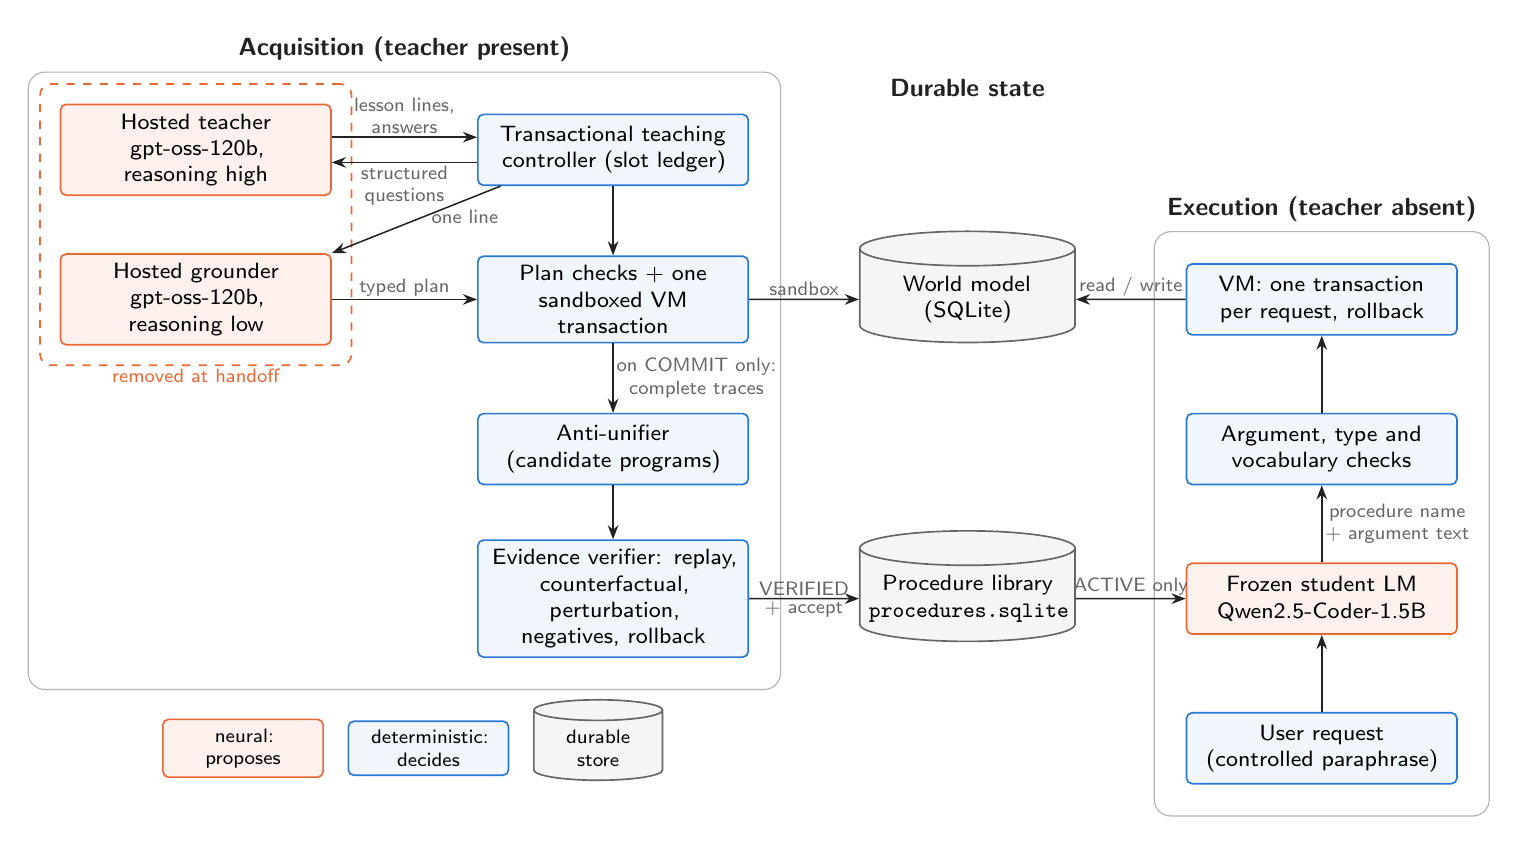
\begin{tikzpicture}[
  font=\sffamily\footnotesize,
  neural/.style={draw=semorange, fill=semorange!9, rounded corners=2pt, align=center, minimum height=9mm, text width=32mm, line width=0.6pt},
  det/.style={draw=semblue, fill=semblue!7, rounded corners=2pt, align=center, minimum height=9mm, text width=32mm, line width=0.6pt},
  store/.style={draw=inkmuted, fill=black!4, cylinder, shape border rotate=90, aspect=0.16, align=center, minimum height=12mm, text width=25mm, line width=0.6pt},
  arr/.style={-{Stealth[length=1.8mm]}, line width=0.55pt, draw=ink},
  lab/.style={font=\sffamily\scriptsize, text=inkmuted, align=center, inner sep=1pt},
  sec/.style={font=\sffamily\small\bfseries, text=ink}]
\def\ya{0} \def\yb{-1.9} \def\yc{-3.8} \def\yd{-5.7}
% hosted models
\node[neural] (teacher)  at (0,\ya) {Hosted teacher\\ gpt-oss-120b, reasoning high};
\node[neural] (grounder) at (0,\yb) {Hosted grounder\\ gpt-oss-120b, reasoning low};
% acquisition pipeline
\node[det] (ctrl)   at (5.3,\ya) {Transactional teaching\\ controller (slot ledger)};
\node[det] (sand)   at (5.3,\yb) {Plan checks + one\\ sandboxed VM transaction};
\node[det] (anti)   at (5.3,\yc) {Anti-unifier\\ (candidate programs)};
\node[det] (verify) at (5.3,\yd) {Evidence verifier: replay,\\ counterfactual, perturbation,\\ negatives, rollback};
% stores
\node[store] (world) at (9.8,\yb) {World model\\ (SQLite)};
\node[store] (lib)   at (9.8,\yd) {Procedure library\\ \texttt{procedures.sqlite}};
% execution (flows upward)
\node[det]    (vm)      at (14.3,\yb) {VM: one transaction\\ per request, rollback};
\node[det]    (checks)  at (14.3,\yc) {Argument, type and\\ vocabulary checks};
\node[neural] (student) at (14.3,\yd) {Frozen student LM\\ Qwen2.5-Coder-1.5B};
\node[det]    (req)     at (14.3,-7.6) {User request\\ (controlled paraphrase)};
% acquisition arrows
\draw[arr] ([yshift=1.6mm]teacher.east) -- node[lab, above]{lesson lines,\\ answers} ([yshift=1.6mm]ctrl.west);
\draw[arr] ([yshift=-1.6mm]ctrl.west) -- node[lab, below]{structured\\ questions} ([yshift=-1.6mm]teacher.east);
\draw[arr] (ctrl.south west) ++(3mm,0) -- node[lab, right, pos=0.45]{\,one line} (grounder.north east);
\draw[arr] (grounder) -- node[lab, above]{typed plan} (sand);
\draw[arr] (sand) -- node[lab, right]{on COMMIT only:\\ complete traces} (anti);
\draw[arr] (anti) -- (verify);
\draw[arr] (ctrl) -- (sand);
\draw[arr] (sand) -- node[lab, above]{sandbox} (world);
\draw[arr] (verify) -- node[lab, above]{VERIFIED}  node[lab, below]{+ accept} (lib);
% execution arrows
\draw[arr] (req) -- (student);
\draw[arr] (student) -- node[lab, right]{procedure name\\ + argument text} (checks);
\draw[arr] (checks) -- (vm);
\draw[arr] (lib) -- node[lab, above]{ACTIVE only} (student);
\draw[arr] (vm) -- node[lab, above]{read / write} (world);
% boundaries
\begin{scope}[on background layer]
  \node[draw=semorange, dashed, line width=0.6pt, rounded corners=4pt, fit=(teacher)(grounder), inner sep=2.5mm] (hosted) {};
  \node[lab, text=semorange, anchor=north] at (hosted.south) {removed at handoff};
  \node[draw=inkmuted!50, rounded corners=6pt, fit=(teacher)(grounder)(ctrl)(verify), inner xsep=4mm, inner ysep=4mm] (acq) {};
  \node[sec, anchor=south] at (acq.north) {Acquisition (teacher present)};
  \node[draw=inkmuted!50, rounded corners=6pt, fit=(vm)(req), inner xsep=4mm, inner ysep=4mm] (exe) {};
  \node[sec, anchor=south] at (exe.north) {Execution (teacher absent)};
  \node[sec, anchor=south] at (9.8,0.55) {Durable state};
\end{scope}
% legend
\node[neural, text width=18mm, minimum height=5mm, font=\sffamily\scriptsize] (l1) at (0.6,-7.6) {neural: proposes};
\node[det, text width=18mm, minimum height=5mm, font=\sffamily\scriptsize, right=3mm of l1] (l2) {deterministic: decides};
\node[store, text width=14mm, minimum height=7mm, font=\sffamily\scriptsize, right=3mm of l2] {durable store};
\end{tikzpicture}
}
\caption{\semvm\ architecture in the final (RCI) configuration. Orange components are neural and only propose; blue components are deterministic and decide; grey cylinders are durable stores. The two hosted roles share one frozen gpt-oss-120b checkpoint and are destroyed at handoff. After handoff, requests are interpreted by the frozen 1.5B model and executed only through ACTIVE procedures.}
\label{fig:arch}
\end{figure}

\begin{table}[t]
\centering\small
\caption{Components and authority boundaries (final configuration).}
\label{tab:components}
\begin{tabularx}{\linewidth}{@{}l>{\raggedright}p{2.6cm}>{\raggedright}X>{\raggedright\arraybackslash}X@{}}
\toprule
Component & Implementation & May & May not \\
\midrule
Hosted teacher & gpt-oss-120b, reasoning high, $T{=}0$, max 8{,}192 tokens & write EXAMPLE and STEP lines; answer structured questions & execute anything; see the world state; write the library; survive handoff \\
Hosted grounder & same checkpoint, reasoning low, separate role and cache & map one lesson line (plus the live result list) to a typed plan in JSON & choose among ambiguous referents; emit an unlicensed terminal action; execute \\
Teaching controller & deterministic state machine + slot ledger & order slots, ask questions, commit or abort a demonstration & admit an incomplete or aborted demonstration as evidence \\
Plan checks + VM & deterministic; one SQLite transaction; rollback & validate ops, types, references; execute in the sandbox & run code; execute an unvalidated plan \\
Anti-unifier & deterministic & propose candidate programs from committed traces & propose from uncommitted material or from gold \\
Evidence verifier & deterministic test battery & mark a candidate VERIFIED or REJECTED & consult gold programs or the teacher \\
Procedure library & \id{procedures.sqlite} & store versions, lifecycle, provenance, tests & activate without VERIFIED + explicit accept \\
Frozen student LM & Qwen2.5-Coder-1.5B, frozen & rank ACTIVE procedure names; write argument text & bypass argument, type and vocabulary checks; create or modify procedures \\
Judge (evaluator only) & gpt-oss-120b, separate role & label lesson faithfulness for reporting & influence any system decision \\
\bottomrule
\end{tabularx}
\end{table}

\subsection{State lives outside the context window}\label{sec:querystate}
A conventional LLM agent is monolithic in where it keeps state: the conversation, retrieved documents, tool outputs and intermediate results accumulate in the context window, learned behavior lives in the weights, and the model itself is the only component that reads that state and decides what it means. \semvm\ inverts this (Table~\ref{tab:monolithic}). The world model and the procedure library are the only durable state. No model ever receives the world as text: state is read and written only through typed queries and transactions that the VM executes (FIND, GET, CHILD, SET\_STATUS, \dots), and each neural call receives a small, purpose-built view and returns a typed proposal. In the final configuration:
\begin{itemize}
\item the \textbf{teacher} sees the skill's goal text, its example-value pool, the names and signatures of saved skills, and its own dialogue for the current target; it never sees world rows (median 1{,}310 input tokens over the 212 cached lesson calls of RCI);
\item the \textbf{grounder} sees one instruction, the typed list of results defined so far in the current demonstration (e.g.\ ``\id{r2}: \id{r1} sorted by when (1 element)''), the primitive inventory and ACTIVE signatures, with no dialogue history (median 4{,}488 input tokens over 768 calls, most of it the fixed card and few-shot examples);
\item the \textbf{student model at reuse} sees a fixed few-shot block, the signatures (name, typed parameters, return type) of ACTIVE procedures and the request, and ranks names or writes an argument list; it never sees the procedures' bodies or the world.
\end{itemize}
Because the context carries references (\id{r1}, \id{request:000011}) rather than contents, its size depends on the instruction and the protocol, not on how large the world is or how many turns have passed; what the model ``knows'' about the world at any step is exactly what a query returned. Every answer can therefore be traced to specific rows, transactions and procedure versions, a model cannot silently alter state, and nothing depends on a transcript surviving a restart---the property that the handoff exploits. Earlier experiments in the project tested this placement directly at larger scale (Appendix~\ref{app:history}): a store scaled from 1K to 1M records at a constant working set, a 64-turn closed loop at about 24 model-facing tokens per turn against a transcript that grew to 1{,}306, and a frozen backbone reading a 512-entity store through typed operations at 29.2 tokens per turn, where a context-stuffing baseline needed about 20{,}000 tokens and failed (a comparison its report notes is confounded with out-of-distribution length). Those results are background, not evidence released here. In the bounded worlds of this paper the relevant observation is architectural: none of the prompts above contains world state by construction.

\begin{table}[t]
\centering\small
\caption{Where state lives: a monolithic LLM agent versus \semvm.}
\label{tab:monolithic}
\begin{tabularx}{\linewidth}{@{}>{\raggedright}p{3.1cm}>{\raggedright}X>{\raggedright\arraybackslash}X@{}}
\toprule
 & Monolithic LLM agent & \semvm \\
\midrule
Working state & tokens in the context window (conversation, tool outputs, retrieved text) & rows in a SQLite world model, read through typed queries; context holds references \\
Learned skills & weights (fine-tuning) or prompt text & versioned, verified programs in \id{procedures.sqlite} \\
Who executes & the model, token by token & a deterministic VM, one transaction per request \\
Who decides what changes & the model & deterministic checks, verifier and explicit accept \\
Growth with history & context grows with turns and retrieved content & context bounded by protocol; state grows on disk \\
After restart & state must be re-supplied in context & state and skills persist; the model is reloaded unchanged \\
Audit & inspect a transcript & state hashes, transaction diffs, test records, provenance \\
\bottomrule
\end{tabularx}
\end{table}

\subsection{World model and VM}
The domain is a personal organizer: events REMINDER, REQUEST, PLAN and NOTE, each optionally about an item CALL, EMAIL, VISIT or MESSAGE; relations WHO, RECIPIENT, WHEN, WHERE and TOPIC; and an open/closed status. The world is a SQLite store with persistent identifiers (\id{request:000011}), canonical state hashing and an audit table. Every request or teaching slot executes as a transaction with postconditions and rollback on failure; the VM executes a frozen inventory of 21 typed primitives (e.g.\ FIND, FILTER, SORT, FIRST, COUNT, SET\_STATUS, FOR, CALL, RETURN) and no arbitrary code. This runtime was established in the first two experiments of the lineage and carried forward hash-checked thereafter.

\subsection{Procedures and their lifecycle}
A procedure is a typed program over the primitives with named parameters (Figure~\ref{fig:s15}, step 7). Its identity is the hash of its canonical AST. The library stores every version with lifecycle state CANDIDATE $\rightarrow$ TESTING $\rightarrow$ VERIFIED $\rightarrow$ ACTIVE (or REJECTED\_*), its source interactions and trace hashes, the proposer, and every test result; an \id{active_pointer} table names the one executable version (Figure~\ref{fig:lifecycle}b). Rejected versions are retained but can never be executed.

\subsection{Evidence verifier}\label{sec:verifier}
Candidates are judged only against evidence from committed traces, never against gold. The battery (Table~\ref{tab:verifier}) consists of static validation; interface checks; replay of each source trace; counterfactual argument substitution, where the reference is the \emph{unabstracted} trace with values substituted; state perturbations (e.g.\ all events closed, alternate events closed) that expose dropped constant filters; negative cases (missing input, wrong type, empty result, ambiguous entity, deleted object, empty world); rollback injection after every state-changing step; and determinism. The perturbation stage was added before any development run of the second experiment, after the unit suite showed that a verifier without it accepted a candidate that dropped a constant \id{STATUS=OPEN} filter because every evidence state happened to have all events open. The general lesson is that an evidence-only verifier can only be as discriminating as the diversity of the states it is allowed to test in.

\subsection{Transactional teaching}
A lesson is an EXAMPLE line giving the example parameter values, followed by STEP lines. The controller turns the lesson into a slot ledger and runs the state machine of Figure~\ref{fig:lifecycle}a. Its registered rules include: an EXAMPLE is required before any step executes; a terminal RETURN is licensed only on the last slot and only when the goal asks for an output; saved skills are called only by name with explicit inputs; if more than one live result could fill a reference, the student asks a structured question listing the legal referents and accepts only \texttt{REFERENT: <id>}; grammar-legality feedback (e.g.\ an inner event's time is \id{PARENT.WHEN}) is returned on rejection; lines injected by the evaluator are never presented to the teacher as the teacher's own; and a demonstration commits only if the completeness check finds no unexecuted slot. An abort restores the sandbox snapshot and contributes zero evidence. Budgets are fixed per target (Appendix~\ref{app:gates}).

\begin{figure}[t]
\centering
\resizebox{\linewidth}{!}{% Figure 2: demonstration transaction state machine (top) and procedure lifecycle (bottom)
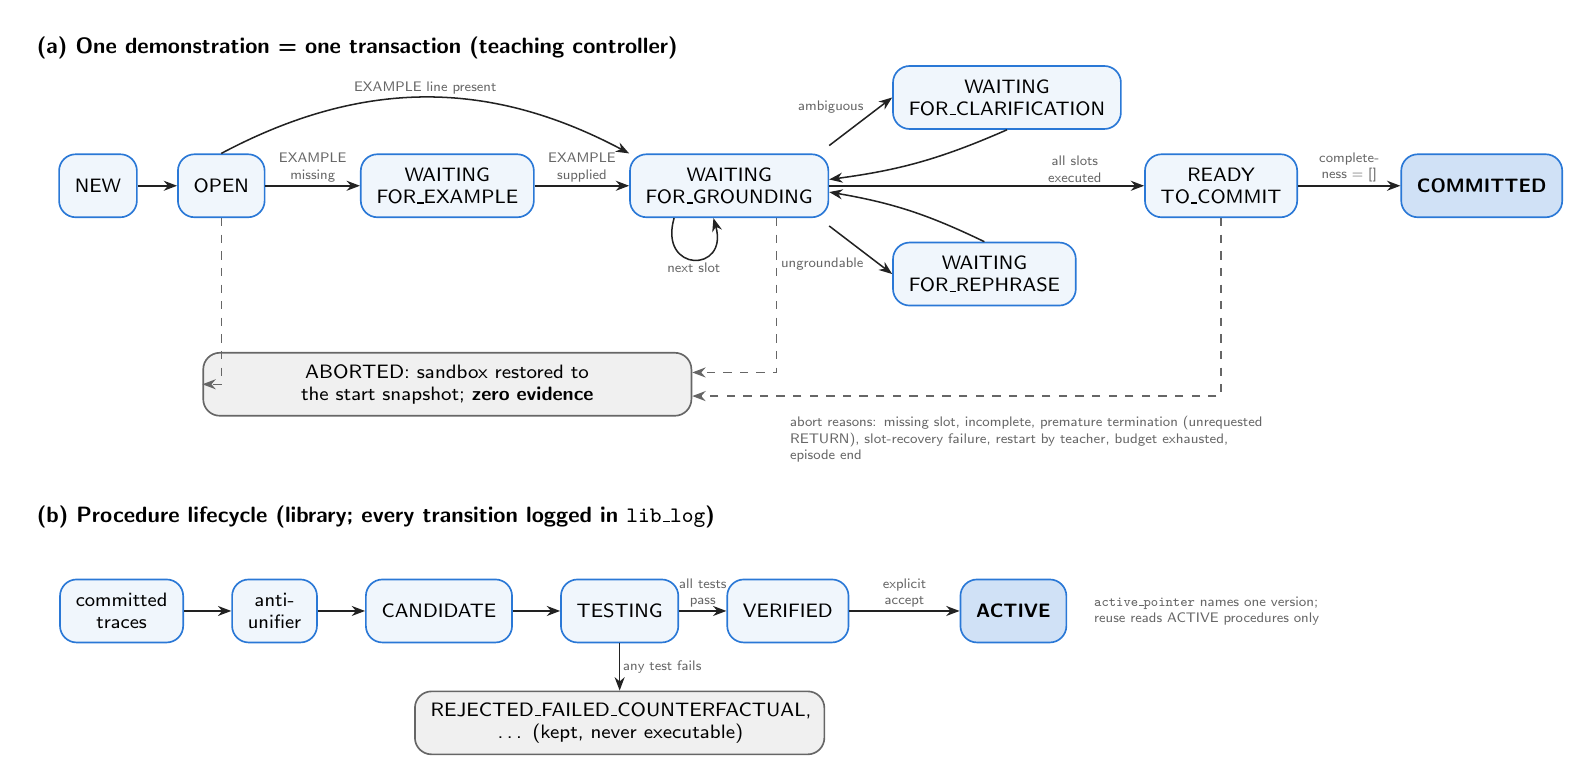
\begin{tikzpicture}[
  font=\sffamily\scriptsize,
  st/.style={draw=semblue, fill=semblue!7, rounded corners=6pt, align=center, minimum height=8mm, inner xsep=2mm, line width=0.6pt},
  good/.style={st, draw=semblue, fill=semblue!22, font=\sffamily\scriptsize\bfseries},
  bad/.style={st, draw=inkmuted, fill=black!6},
  arr/.style={-{Stealth[length=1.7mm]}, line width=0.55pt, draw=ink},
  lab/.style={font=\sffamily\tiny, text=inkmuted, align=center, inner sep=1pt},
  sec/.style={font=\sffamily\footnotesize\bfseries, anchor=west}]
% ---- row 1
\node[sec] at (-0.9,1.75) {(a) One demonstration = one transaction (teaching controller)};
\node[st] (new) at (0,0) {NEW};
\node[st, right=5mm of new] (open) {OPEN};
\node[st, right=12mm of open] (ex) {WAITING\\FOR\_EXAMPLE};
\node[st, right=12mm of ex] (gr) {WAITING\\FOR\_GROUNDING};
\node[st, above right=3mm and 8mm of gr] (cl) {WAITING\\FOR\_CLARIFICATION};
\node[st, below right=3mm and 8mm of gr] (re) {WAITING\\FOR\_REPHRASE};
\node[st, right=40mm of gr] (ready) {READY\\TO\_COMMIT};
\node[good, right=13mm of ready] (com) {COMMITTED};
\node[bad, below=17mm of ex, text width=58mm] (ab) {ABORTED: sandbox restored to the start snapshot; \textbf{zero evidence}};
\draw[arr] (new) -- (open);
\draw[arr] (open) -- node[lab, above]{EXAMPLE\\ missing} (ex);
\draw[arr] (ex) -- node[lab, above]{EXAMPLE\\ supplied} (gr);
\draw[arr] (open.north) to[bend left=28] node[lab, above]{EXAMPLE line present} (gr.north west);
\draw[arr] ($(gr.south)+(-7mm,0)$) .. controls +(-2mm,-7mm) and +(2mm,-7mm) .. node[lab, below]{next slot} ($(gr.south)+(-2mm,0)$);
\draw[arr] ([yshift=1mm]gr.north east) -- node[lab, above left, pos=0.6]{ambiguous} (cl.west);
\draw[arr] (cl.south) to[bend left=8] ([yshift=0.8mm]gr.east);
\draw[arr] ([yshift=-1mm]gr.south east) -- node[lab, below left, pos=0.6]{ungroundable} (re.west);
\draw[arr] (re.north) to[bend right=8] ([yshift=-0.8mm]gr.east);
\draw[arr] (gr.east) -- node[lab, above, pos=0.78]{all slots\\ executed} (ready.west);
\draw[arr] (ready) -- node[lab, above]{complete-\\ness = []} (com);
\draw[arr, draw=inkmuted, dashed] (open.south) |- (ab.west);
\draw[arr, draw=inkmuted, dashed] ($(gr.south)+(6mm,0)$) |- ($(ab.east)+(0,1.5mm)$);
\draw[arr, draw=inkmuted, dashed] (ready.south) |- ($(ab.east)+(0,-1.5mm)$);
\node[lab, anchor=west, text width=60mm, align=left] at ($(ab.east)+(12mm,-7mm)$) {abort reasons: missing slot, incomplete, premature termination (unrequested RETURN), slot-recovery failure, restart by teacher, budget exhausted, episode end};
% ---- row 2
\def\yy{-5.4}
\node[sec] at (-0.9,\yy+1.2) {(b) Procedure lifecycle (library; every transition logged in \texttt{lib\_log})};
\node[st] (tr) at (0.3,\yy) {committed\\ traces};
\node[st, right=6mm of tr] (au) {anti-\\unifier};
\node[st, right=6mm of au] (cand) {CANDIDATE};
\node[st, right=6mm of cand] (test) {TESTING};
\node[st, right=6mm of test] (ver) {VERIFIED};
\node[good, right=14mm of ver] (act) {ACTIVE};
\node[bad, below=6mm of test, text width=48mm] (rej) {REJECTED\_FAILED\_COUNTERFACTUAL, \dots\ (kept, never executable)};
\node[lab, right=3mm of act, text width=30mm, align=left] {\texttt{active\_pointer} names one version; reuse reads ACTIVE procedures only};
\draw[arr] (tr) -- (au); \draw[arr] (au) -- (cand); \draw[arr] (cand) -- (test);
\draw[arr] (test) -- node[lab, above]{all tests\\ pass} (ver);
\draw[arr] (ver) -- node[lab, above]{explicit\\ accept} (act);
\draw[arr] (test) -- node[lab, right]{any test fails} (rej);
\end{tikzpicture}
}
\caption{(a) A demonstration is one transaction: only COMMITTED demonstrations become learning evidence; any abort restores the sandbox and yields zero evidence. (b) Procedure lifecycle in the library: activation requires every verifier test to pass and an explicit accept.}
\label{fig:lifecycle}
\end{figure}

\subsection{Handoff and reuse}
After acquisition the hosted app is stopped, the endpoint is probed (the registered requirement is HTTP 404 / unavailable), lesson transcripts and teaching context are removed from the student's directory, teacher credentials are scrubbed from the environment, and every subsequent process runs under a network guard that blocks non-loopback connections and logs attempts (Figure~\ref{fig:handoff}). Reuse requests use wording that did not appear in the lesson and, where registered, arguments never demonstrated, and are interleaved with process restarts. A request is served by (i) a deterministic alias rule or (ii) the frozen 1.5B model ranking the ACTIVE procedure names by log-probability with a registered margin of 1.0 nats, below which the system clarifies; the model then writes the argument list, which must pass type, vocabulary and presence checks, with a typed fallback; otherwise the system clarifies.

\begin{figure}[t]
\centering
\resizebox{\linewidth}{!}{% Figure 3: teacher removal and persistence (swimlane timeline)
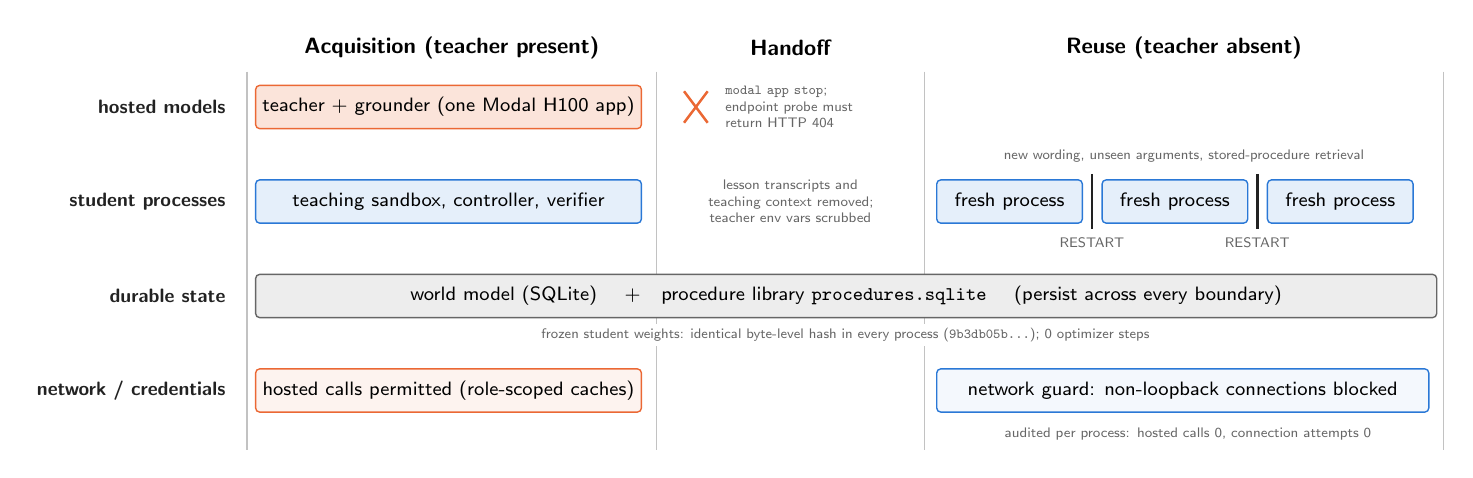
\begin{tikzpicture}[font=\sffamily\scriptsize,
  lane/.style={font=\sffamily\scriptsize\bfseries, anchor=east, align=right, text=ink},
  bar/.style={rounded corners=1.5pt, minimum height=5.5mm, align=center, inner sep=1pt, line width=0.5pt},
  hb/.style={bar, draw=semorange, fill=semorange!18},
  sb/.style={bar, draw=semblue, fill=semblue!12},
  db/.style={bar, draw=inkmuted, fill=black!7},
  mk/.style={draw=ink, line width=0.9pt},
  lab/.style={font=\sffamily\tiny, text=inkmuted, align=center}]
\def\xa{0} \def\xb{5.2} \def\xc{8.6} \def\xe{15.2}
% phase headers
\foreach \x/\y/\t in {\xa/\xb/Acquisition (teacher present), \xb/\xc/Handoff, \xc/\xe/Reuse (teacher absent)}{
  \node[font=\sffamily\footnotesize\bfseries] at ({(\x+\y)/2}, 0.75) {\t};
  \begin{scope}[on background layer]\draw[inkmuted!40] (\x,0.45) -- (\x,-4.35);\end{scope}}
\begin{scope}[on background layer]\draw[inkmuted!40] (\xe,0.45) -- (\xe,-4.35);\end{scope}
% lanes
\node[lane] at (-0.15,0) {hosted models};
\node[lane] at (-0.15,-1.2) {student processes};
\node[lane] at (-0.15,-2.4) {durable state};
\node[lane] at (-0.15,-3.6) {network / credentials};
% hosted lane
\node[hb, minimum width=4.9cm, anchor=west] at (0.1,0) {teacher + grounder (one Modal H100 app)};
\draw[mk, semorange] (5.55,-0.2) -- (5.85,0.2) (5.55,0.2) -- (5.85,-0.2);
\node[lab, anchor=west, text width=2.7cm, align=left] at (5.95,0) {\texttt{modal app stop};\\ endpoint probe must\\ return HTTP 404};
% student lane
\node[sb, minimum width=4.9cm, anchor=west] at (0.1,-1.2) {teaching sandbox, controller, verifier};
\node[lab, text width=3.1cm] at ({(\xb+\xc)/2},-1.2) {lesson transcripts and\\ teaching context removed;\\ teacher env vars scrubbed};
\node[sb, minimum width=1.85cm, anchor=west] at (8.75,-1.2) {fresh process};
\node[sb, minimum width=1.85cm, anchor=west] at (10.85,-1.2) {fresh process};
\node[sb, minimum width=1.85cm, anchor=west] at (12.95,-1.2) {fresh process};
\foreach \x in {10.73, 12.83} {\draw[mk] (\x,-0.85) -- (\x,-1.55); \node[lab] at (\x,-1.72) {RESTART};}
\node[lab] at (11.9,-0.62) {new wording, unseen arguments, stored-procedure retrieval};
% durable lane
\node[db, minimum width=15.0cm, anchor=west] at (0.1,-2.4) {world model (SQLite) \quad+\quad procedure library \texttt{procedures.sqlite} \quad(persist across every boundary)};
\node[lab, fill=white, inner sep=1.5pt] at (7.6,-2.9) {frozen student weights: identical byte-level hash in every process (\texttt{9b3db05b\dots}); 0 optimizer steps};
% network lane
\node[hb, minimum width=4.9cm, anchor=west, fill=semorange!8] at (0.1,-3.6) {hosted calls permitted (role-scoped caches)};
\node[sb, minimum width=6.25cm, anchor=west, fill=semblue!5] at (8.75,-3.6) {network guard: non-loopback connections blocked};
\node[lab, text width=6.2cm] at (11.95,-4.15) {audited per process: hosted calls 0, connection attempts 0};
\end{tikzpicture}
}
\caption{Teacher removal and persistence. Only the world model and procedure library cross the handoff; the frozen student's weight hash is checked in every process. The LOCKED run's handoff probe returned HTTP 401 rather than 404 (Section~\ref{sec:locked}).}
\label{fig:handoff}
\end{figure}

\subsection{Evaluation vocabulary}
All metrics are computed by an evaluator that uses an independent oracle interpreter. The primary metrics are: \textbf{learned procedure exact} (the ACTIVE program for a target has the same canonical hash as the registered reference program; behaviorally equivalent variants count as failures); \textbf{scenario exact} (every acquisition and post-handoff turn of the scenario matches the oracle, including world state); \textbf{distilled skill exact} (a target is acquired, verified, activated, the teacher is verifiably destroyed, and every post-handoff invocation is exact with zero hosted calls); and \textbf{grounding behavioral exact} (a grounded demonstration is behaviorally equivalent to the reference for its own example values across five registered worlds). Safety metrics count wrong committed actions, incomplete or aborted evidence committed, unrequested terminal actions executed, ambiguous references executed and bad procedures activated. Gates were registered before each run; we report numerators and denominators throughout.

\section{Research progression}\label{sec:lineage}

Figure~\ref{fig:progression} and Table~\ref{tab:lineage} summarize the seven experiments. Each was specified in a preregistration document with gates, stop rules and a sealed LOCKED set; each stopped at its registered decision point. About six weeks of earlier preregistered experiments (Appendix~\ref{app:history}; code and results not part of this release) are not part of this paper's evidence; their main influence was a repeated observation that multi-step bookkeeping fails when left inside a network and becomes exact when made explicit in a deterministic runtime, and that a small controller can act over a large store at constant context when it reaches state through typed queries.

\begin{figure}[t]
\centering
\resizebox{\linewidth}{!}{% Figure 4: research progression (each row: what was added, what was observed, what remained)
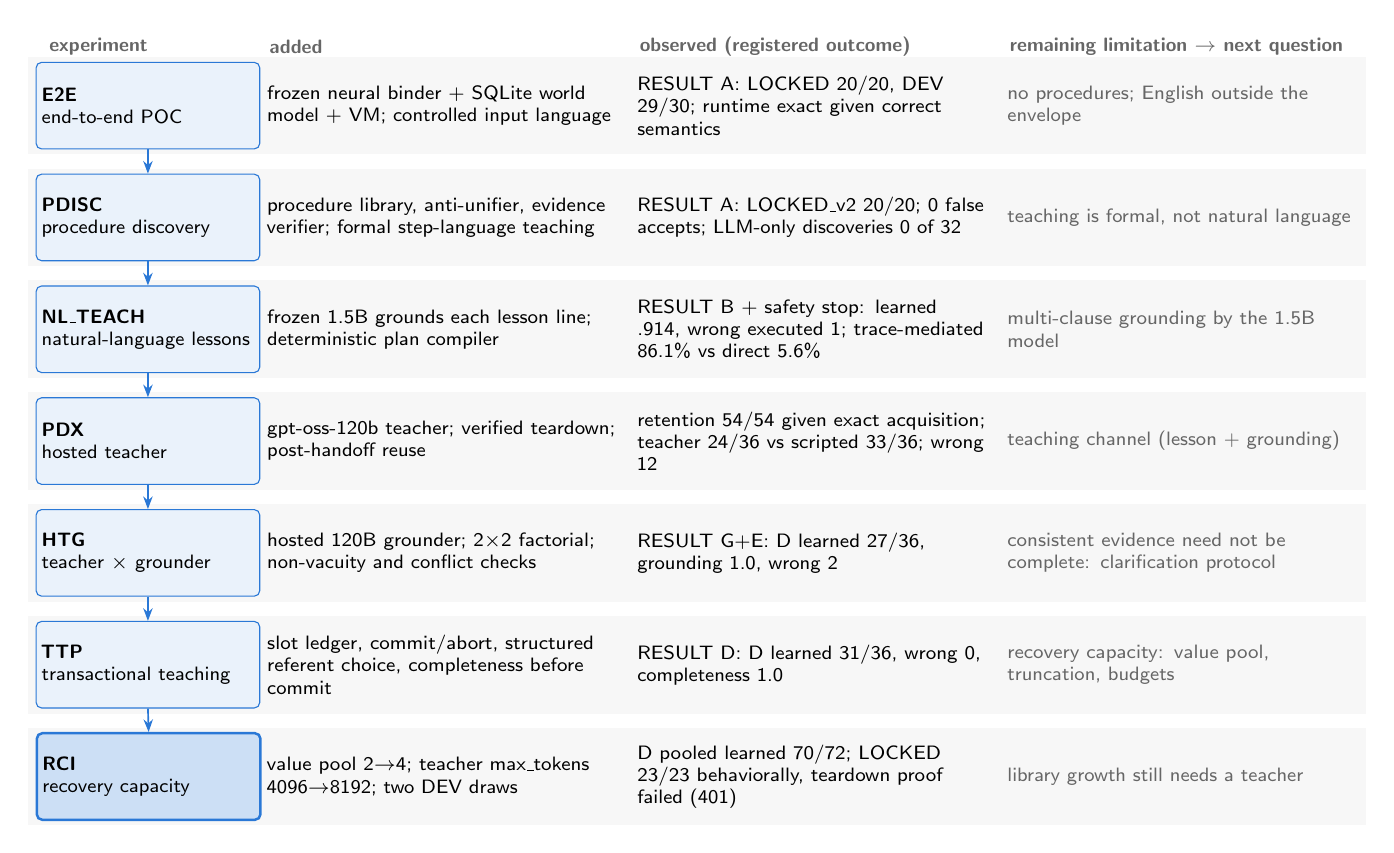
\begin{tikzpicture}[font=\sffamily\scriptsize,
  exp/.style={draw=semblue, fill=semblue!10, rounded corners=2pt, text width=27mm, minimum height=11mm, align=left, inner sep=2pt, font=\sffamily\scriptsize},
  fin/.style={exp, fill=semblue!24, line width=0.9pt},
  cell/.style={text width=44mm, align=left, execute at begin node={\hyphenpenalty=10000\exhyphenpenalty=10000}, inner sep=1pt, font=\sffamily\scriptsize},
  hdr/.style={font=\sffamily\scriptsize\bfseries, text=inkmuted, anchor=west},
  arr/.style={-{Stealth[length=1.6mm]}, line width=0.6pt, draw=semblue}]
\node[hdr] at (-1.45,0.75) {experiment};
\node[hdr] at (1.35,0.75) {added};
\node[hdr] at (6.05,0.75) {observed (registered outcome)};
\node[hdr] at (10.75,0.75) {remaining limitation $\rightarrow$ next question};
\def\rowgap{1.42}
\foreach \i/\n/\a/\o/\r [count=\k] in {
  0/{\textbf{E2E}\\ end-to-end POC}/{frozen neural binder + SQLite world model + VM; controlled input language}/{RESULT A: LOCKED \eepLocked, DEV \eepDev; runtime exact given correct semantics}/{no procedures; English outside the envelope},
  1/{\textbf{PDISC}\\ procedure discovery}/{procedure library, anti-unifier, evidence verifier; formal step-language teaching}/{RESULT A: LOCKED\_v2 \pdLocked; 0 false accepts; LLM-only discoveries \pdLlmOnly\ of \pdDiscoveries}/{teaching is formal, not natural language},
  2/{\textbf{NL\_TEACH}\\ natural-language lessons}/{frozen 1.5B grounds each lesson line; deterministic plan compiler}/{RESULT B + safety stop: learned \nlLearned, wrong executed \nlWrongExec; trace-mediated \nlTrace\% vs direct \nlDirect\%}/{multi-clause grounding by the 1.5B model},
  3/{\textbf{PDX}\\ hosted teacher}/{gpt-oss-120b teacher; verified teardown; post-handoff reuse}/{retention \pdxRetention\ given exact acquisition; teacher \pdxTeacherLearned\ vs scripted \pdxScriptedLearned; wrong \pdxWrong}/{teaching channel (lesson + grounding)},
  4/{\textbf{HTG}\\ teacher $\times$ grounder}/{hosted 120B grounder; 2$\times$2 factorial; non-vacuity and conflict checks}/{RESULT G+E: D learned \htgDLearned, grounding \htgDGround, wrong \htgDWrong}/{consistent evidence need not be complete: clarification protocol},
  5/{\textbf{TTP}\\ transactional teaching}/{slot ledger, commit/abort, structured referent choice, completeness before commit}/{RESULT D: D learned \ttpDLearned, wrong \ttpDWrong, completeness 1.0}/{recovery capacity: value pool, truncation, budgets},
  6/{\textbf{RCI}\\ recovery capacity}/{value pool 2$\rightarrow$4; teacher max\_tokens 4096$\rightarrow$8192; two DEV draws}/{D pooled learned \rciDLearnedPooled; LOCKED \lockedLearned\ behaviorally, teardown proof failed (401)}/{library growth still needs a teacher}}{
  \pgfmathsetmacro\y{-\i*\rowgap}
  \ifnum\k=7 \node[fin, anchor=west] (e\k) at (-1.5,\y) {\n}; \else \node[exp, anchor=west] (e\k) at (-1.5,\y) {\n}; \fi
  \node[cell, anchor=west] at (1.4,\y) {\a};
  \node[cell, anchor=west] at (6.1,\y) {\o};
  \node[cell, anchor=west, text=inkmuted] at (10.8,\y) {\r};
  \begin{scope}[on background layer]\fill[black!3] (-1.6,\y-0.62) rectangle (15.4,\y+0.62);\end{scope}
}
\foreach \k [evaluate=\k as \kk using int(\k+1)] in {1,...,6} {\draw[arr] (e\k.south) -- (e\kk.north);}
\end{tikzpicture}
}
\caption{Research progression. Each experiment added one layer and was stopped at its registered decision point; the residual limitation of each became the next question.}
\label{fig:progression}
\end{figure}

\begin{table}[t]
\centering\small
\caption{Experiment lineage. Outcome labels are those registered in each experiment's own preregistration. ``LOCKED'' is the sealed test set; ``not run'' means the registered stop rule fired on DEV and the sealed set stayed unopened.}
\label{tab:lineage}
\begin{tabularx}{\linewidth}{@{}l>{\raggedright}p{3.6cm}>{\raggedright}X>{\raggedright\arraybackslash}p{2.1cm}@{}}
\toprule
Experiment & Question & Key observed numbers & LOCKED \\
\midrule
E2E & Does a frozen binder + deterministic VM form a working persistent runtime? & DEV scenarios \eepDev; binder errors only (1 parent-binding error) & run once: \eepLocked \\
PDISC & Can procedures be induced from traces and reused after restart? & 0 false accepts on bad candidates; LLM-only discoveries \pdLlmOnly\ of \pdDiscoveries & run once: \pdLocked \\
NL\_TEACH & Can a frozen 1.5B model ground natural-language lessons? & learned \nlLearned; scenario \nlScenario; wrong executed \nlWrongExec; false accept \nlFalseAccept; trace-mediated \nlTrace\% vs direct \nlDirect\% & not run \\
PDX & Can a hosted 120B teacher teach the frozen student? & teacher learned \pdxTeacherLearned\ vs scripted \pdxScriptedLearned; wrong \pdxWrong; false accept \pdxFalseAccept; retention \pdxRetention & not run \\
HTG & Does a hosted grounder fix the teaching channel? & Arm D learned \htgDLearned; grounding \htgDGround; wrong \htgDWrong & not run \\
TTP & Does a transactional protocol remove unsafe acquisition? & Arm D learned \ttpDLearned; wrong \ttpDWrong; completeness 1.0 & not run \\
RCI & Is the residual recovery capacity? & Arm D pooled learned \rciDLearnedPooled; scenario \rciDScenarioPooled; wrong 0 & run once: \lockedLearned\ learned; not a clean pass \\
\bottomrule
\end{tabularx}
\end{table}

\paragraph{E2E (END\_TO\_END\_POC\_V1).} A small frozen neural binder from earlier work (checkpoint hash-pinned) translated a controlled compositional language with multiple modifier bindings into a canonical intermediate representation, which a deterministic resolver and VM applied to the SQLite world. RESULT A within the registered regime: LOCKED \eepLocked\ scenarios exact, DEV \eepDev\ (the single miss was one neural parent-binding error), and the gold-IR control exact on both suites. The input language was a controlled, tag-coindexed language; English was out of scope and rejected (0/8 exact, 8/8 rejected by the envelope check).

\paragraph{PDISC (PROCEDURE\_DISCOVERY\_POC\_V1).} Added the procedure library, deterministic anti-unification and the evidence verifier, with teaching in a formal step language and retrieval by controlled paraphrase. RESULT A: LOCKED\_v2 \pdLocked\ with every registered gate at 1.0, and 0 of 6 deliberately bad candidates accepted. The frozen 1.5B model was also asked to propose procedures: every procedure it got right, anti-unification also got right (\pdLlmOnly\ LLM-only verified discoveries of \pdDiscoveries\ on LOCKED). It was load-bearing for retrieval ranking, not for induction. A first LOCKED set was invalidated before being run after a scenario-design defect was found on DEV, and a fresh one was sealed.

\paragraph{NL\_TEACH.} Replaced formal teaching with natural-language lessons grounded by the frozen 1.5B model through grammar-constrained ranking of legal typed options and a deterministic multi-clause plan compiler. RESULT B with a safety stop after three registered DEV iterations: learned \nlLearned, scenario \nlScenario, \nlWrongExec\ wrong action executed (\nlWrongProposed\ wrong raw proposals, \nlWrongBlocked\ blocked or repaired), and \nlFalseAccept\ verifier false accept caused upstream by a lost second demonstration. The strongest observation was methodological: the same model writing the program directly from the lesson was exact for \nlDirect\% of procedures, while trace-mediated learning was exact for \nlTrace\%. LOCKED was not run.

\paragraph{PDX (hosted teacher).} Introduced a hosted gpt-oss-120b teacher and the handoff protocol. Retention was positive: every exactly acquired skill was reused exactly after the teacher was destroyed (\pdxRetention\ invocations). Acquisition was negative: the hosted teacher reached \pdxTeacherLearned\ learned procedures against \pdxScriptedLearned\ from fixed scripted lessons, with \pdxWrong\ wrong executed demonstrations, split roughly evenly between teacher-side errors (unrequested constraints) and student-side mis-grounding. Two DEV attempts were superseded before the final one (a scenario-design defect; truncation of 32/98 teacher replies at a 1{,}200-token cap). LOCKED was not run.

\paragraph{HTG (hosted teacher $\times$ grounder).} A $2\times2$ of teacher (scripted vs hosted) and grounder (local 1.5B vs hosted 120B), with added evidence non-vacuity and conflict checks. Arm D (hosted $\times$ hosted) had grounding behavioral exact \htgDGround\ but learned only \htgDLearned\ and executed \htgDWrong\ wrong actions. Both wrong actions share a lesson that we carry forward: \emph{consistent evidence is not necessarily complete evidence}. In one, an unrequested RETURN ended a demonstration after one step and a one-step wrapper verified against that truncated evidence; in the other, an injected vague step was never restored and the resulting program returned calls instead of people. The verifier behaved as specified in both cases. The bottleneck had moved from grounding accuracy to the clarification protocol. LOCKED was not run.

\paragraph{TTP (transactional teaching).} Treated a demonstration as a transaction (Figure~\ref{fig:lifecycle}a) and fixed each HTG failure class in general form. Arm D passed every safety gate (0 wrong actions, 0 incomplete commits, completeness 1.0, 5 unrequested RETURNs blocked) but not accuracy: learned \ttpDLearned\ (.861), scenario .833. The five misses were attributed to provider truncation at 4{,}096 tokens, a two-value teacher pool that could not survive a rejected legal-bad demonstration, a per-target turn budget, and one false clarification (RESULT D). The first FINAL\_DEV attempt was invalid and archived (Section~\ref{sec:integrity}). LOCKED was not run.

\paragraph{RCI (recovery capacity isolation).} The centerpiece, described next.

\section{Recovery capacity isolation}\label{sec:rci}

\subsection{Design}
RCI asked whether TTP's residual failures required a new recovery architecture or only more resources. The controller, prompts, grounder, verifier, budgets and thresholds were inherited unchanged, with TTP's post-run Amendment~003 (count committed demonstrations, not indices) as the baseline rather than a treatment.

\paragraph{Stage 0.} (A) A parity audit using only generator source and manifest metadata found that the parent's sealed LOCKED set embedded a two-value teacher pool at generation time, so a successor LOCKED set was generated from the same never-inspected blind templates with a new seed and sealed before any RCI development run. (B) A failure taxonomy with an earliest-cause rule and fixed precedence (teacher $\rightarrow$ grounder $\rightarrow$ controller $\rightarrow$ evidence $\rightarrow$ procedure) was frozen before scoring. (C) A non-confirmatory ceiling diagnostic re-ran the five parent Arm D failures with relaxed budgets; \rciCeiling\ recovered exactly, which was the registered go signal.

\paragraph{Stage 1 intervention.} Exactly two settings changed: the teacher example-value pool from 2 to 4 values per class (each with witness events), and the teacher \id{max_tokens} from 4{,}096 to 8{,}192. The serving context length was raised from 16{,}384 to 32{,}768 only so that these budgets fit; it is a serving parameter with the same checkpoint and sampling. The configuration fingerprint (\id{dacd7a90...}) was frozen before the first development draw and is identical in both draws and in LOCKED.

\paragraph{Factorial.} All four arms used the same hosted grounder. Lesson source was scripted (registered lessons) or hosted (the teacher); recovery source (the answers to rephrase and reference questions) was scripted (a frozen lookup of registered rephrasings), hosted (a separately cached recovery-teacher role), or oracle (answers derived from the registered reference program, and only when the executed prefix matched it). Arm D (hosted lesson, hosted recovery) was the confirmatory arm; B, E and F were attribution arms. Two development draws (DEV-A, DEV-B; 30 scenarios and 36 targets each; 20 strata) were run with no change of any kind between them. Primary gates were pooled with per-replicate floors of .80, and safety gates had to hold in each replicate independently.

\subsection{Results}

\begin{table}[t]
\centering\small
\caption{Parent (TTP) versus successor (RCI) for Arm D. The parent row is its own DEV draw; the RCI rows are two further independent draws. Draws differ, so the comparison is indicative, not paired.}
\label{tab:parent}
\begin{tabular}{lrrl}
\toprule
Metric (Arm D) & TTP parent & RCI pooled & RCI DEV-A / DEV-B\\
\midrule
Learned procedure exact & 31/36 (.861) & 70/72 (.972) & 36/36 \;/\; 34/36\\
Scenario exact & 25/30 (.833) & 58/60 (.967) & 30/30 \;/\; 28/30\\
Distilled skill exact & 27/32 (.844) & 62/64 (.969) & 32/32 \;/\; 30/32\\
Grounding behavioral exact & 32/38 (.842) & 71/71 (1.0) & 36/36 \;/\; 35/35\\
Wrong committed actions & 0 & 0 & 0 \;/\; 0\\
\bottomrule
\end{tabular}

\end{table}

\begin{table}[t]
\centering\small
\caption{RCI factorial, all arms with the hosted 120B grounder. Cells are DEV-A + DEV-B = pooled. The grounding column uses the registered gate definition, which also counts faithful demonstrations that were later aborted.}
\label{tab:factorial}
\resizebox{\linewidth}{!}{\begin{tabular}{llrrrr}
\toprule
Arm & Lesson / recovery & Learned & Scenario & Distilled & Grounding\\
\midrule
B & scripted / scripted & 36/36 + 35/36 = \textbf{71/72} & 30/30 + 29/30 = \textbf{59/60} & 32/32 + 31/32 = \textbf{63/64} & 36/37 + 35/41 = \textbf{71/78}\\
E & scripted / hosted & 36/36 + 36/36 = \textbf{72/72} & 30/30 + 30/30 = \textbf{60/60} & 32/32 + 32/32 = \textbf{64/64} & 36/36 + 36/36 = \textbf{72/72}\\
F & hosted / oracle & 34/36 + 34/36 = \textbf{68/72} & 28/30 + 28/30 = \textbf{56/60} & 30/32 + 30/32 = \textbf{60/64} & 35/35 + 37/38 = \textbf{72/73}\\
D & hosted / hosted & 36/36 + 34/36 = \textbf{70/72} & 30/30 + 28/30 = \textbf{58/60} & 32/32 + 30/32 = \textbf{62/64} & 36/36 + 35/35 = \textbf{71/71}\\
\bottomrule
\end{tabular}
}
\end{table}

\begin{figure}[t]
\centering
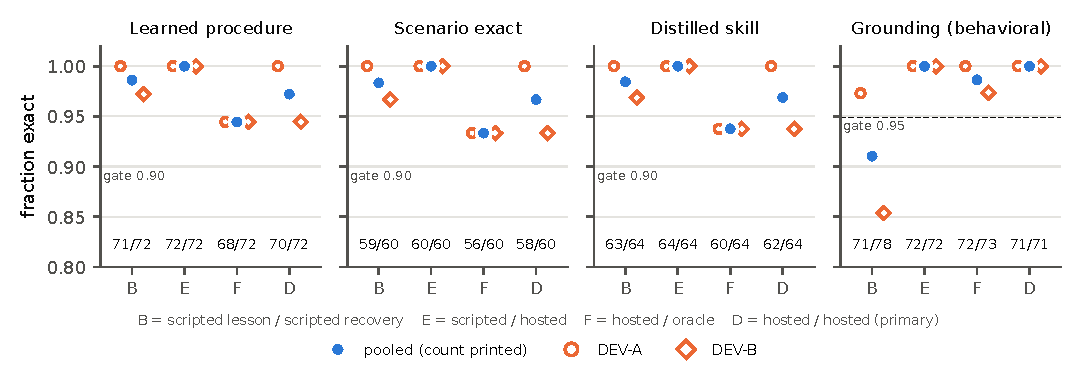
\includegraphics[width=\linewidth]{figures/fig_factorial.pdf}
\caption{RCI factorial: pooled rates (filled) and per-replicate rates (hollow) with counts; dashed lines are Arm D's registered gates. The vertical axis starts at 0.8; all differences between arms are a few targets.}
\label{fig:factorial}
\end{figure}

\paragraph{Arm D passes every pooled gate.} Pooled over both draws, Arm D learned \rciDLearnedPooled\ procedures exactly (registered minimum \rciDLearnedMin), with \rciDScenarioPooled\ exact scenarios (minimum \rciDScenarioMin), \rciDDistilledPooled\ distilled skills (minimum \rciDDistilledMin) and \rciDGroundingPooled\ grounding (minimum \rciDGroundingMin); per replicate the values were \rciDLearnedA\ and \rciDLearnedB\ learned (Table~\ref{tab:parent}). In each replicate there were zero wrong committed actions, zero incomplete commits, zero unrequested or ambiguous executions and zero bad activations; replay, counterfactual, rollback and reuse given acquisition were all 1.0; the teardown probe returned 404 in both draws. For orientation only, descriptive 95\% Wilson intervals are [.904, .992] for pooled learned (70/72) and [.886, .991] for pooled scenario (58/60); no significance test is implied. Hosted-teacher truncations fell from 9 in the parent Arm D to 0, and no pool-exhaustion failure occurred.

\paragraph{Residual failures.} DEV-A had none. DEV-B had one TEACHER\_INITIAL\_SEMANTIC\_ERROR and one EVIDENCE\_NONVACUITY\_FAILURE. No cause repeated across draws, and the registered trigger for a Stage-2 structured-clarification experiment (mass on grounder false clarification or recovery semantic errors) did not fire.

\paragraph{Factorial interpretation.} Pooled learned counts were B 71/72, E 72/72, F 68/72 and D 70/72 (Table~\ref{tab:factorial}, Figure~\ref{fig:factorial}). We do not rank the arms. Three observations are nonetheless supported by the records:
\begin{itemize}
\item \emph{Scripted recovery, not hosted recovery, was the weak recovery source.} Arm B's scripted recovery replays a registered rephrasing, which the hosted grounder often clarified again: 0 of 14 recovery slots in B grounded, and B recovered by starting new demonstrations instead. The hosted recovery teacher in E resolved 12 of 12 recovery events.
\item \emph{The hosted initial lesson costs a little.} F and D lost two to four targets to initial-lesson content errors, one per replicate; lesson faithfulness as labeled by the judge was .92--.97.
\item \emph{The contrasts are small and their signs do not replicate.} For example, D$-$E on learned was 0 on DEV-A and $-$.056 on DEV-B; the interaction term was $+$.056 and $-$.028. With adequate resources, lesson source and recovery source each moved acquisition by at most about two of 36 targets.
\end{itemize}
The grounding column is lower for B (71/78) because the registered grounding metric counts faithful demonstrations that reached grounding even if they were later aborted. Committed demonstrations were behaviorally exact in every arm and replicate except one in F on DEV-B (44 of 45), the single wrong committed action of the factorial, attributed to a hosted initial-lesson semantic error under oracle recovery.

\begin{figure}[t]
\centering
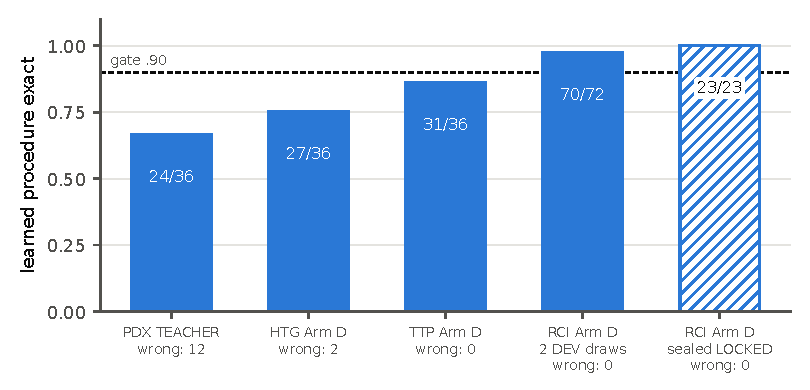
\includegraphics[width=0.92\linewidth]{figures/fig_hosted_arm.pdf}
\caption{Learned-procedure rate of the hosted-teacher arm across the lineage (PDX used the local 1.5B grounder; HTG, TTP and RCI used the hosted grounder). Each bar is a different DEV draw; LOCKED is hatched and, per Section~\ref{sec:locked}, is not a clean pass.}
\label{fig:hostedarm}
\end{figure}

\section{LOCKED evaluation}\label{sec:locked}

The LOCKED scope and pass rule were registered after the pooled decision and before the run: one run of the 20 sealed successor scenarios (23 targets), arms GOLD\_TRACE, FORMAL\_TEACH and D, the identical frozen configuration, and the same thresholds as the pooled gates, with no rerun under any outcome.

\lockedsentence

Table~\ref{tab:locked} lists the criteria as recorded and under the strict registered rule. After LOCKED acquisition, \texttt{modal app stop -{}-yes} returned 0, but the immediate endpoint probe returned HTTP 401: the app was still draining and rejecting unauthenticated requests. The evaluator's teardown helper, inherited from HTG, accepted any HTTP error as ``destroyed'', recorded the teardown as verified, and started reuse. Under the registered rule the teardown-verification gate is 0, and so are the two criteria that depend on it (teacher-disconnect reuse and distilled skill exact). The evidence that the student did not depend on the teacher is strong but is not the registered proof: every reuse process ran with teacher credentials absent and under the network guard, with 0 connection attempts and 0 hosted calls; a later probe returned 404 and the app was listed as stopped; and all reuse results matched the oracle. The same helper had received a real 404 in both development draws and in every earlier experiment's handoff. The helper has since been changed to poll until a real 404 and to reject 401, 403 and 5xx responses; no RCI run used the changed version. LOCKED is not rerun.

\begin{table}[t]
\centering\small
\caption{LOCKED (20 sealed scenarios, 23 targets, Arm D). ``Strict'' applies the registered teardown rule (HTTP 404 required).}
\label{tab:locked}
\resizebox{\linewidth}{!}{\begin{tabular}{lllc}
\toprule
Criterion (Arm D, LOCKED, 20 scenarios) & As recorded & Strict (registered rule) & Gate\\
\midrule
Learned procedure exact & 23/23 & 23/23 & $\ge .90$\\
Scenario exact & 20/20 & 20/20 & $\ge .90$\\
Grounding behavioral exact & 22/23 (.957) & 22/23 & $\ge .95$\\
Wrong committed actions & 0 & 0 & $=0$\\
Incomplete demonstrations committed & 0 & 0 & $=0$\\
Post-handoff hosted calls / network attempts & 0 / 0 & 0 / 0 & $=0$\\
Unseen-arg. / restart / stored reuse given acquisition & 1.0 / 1.0 / 1.0 & 1.0 / 1.0 / 1.0 & $=1$\\
\textbf{Hosted teardown verified} & 1.0 (probe HTTP 401 accepted) & \textbf{0 (401 $\ne$ 404)} & $=1$\\
\textbf{Teacher-disconnect reuse given acquisition} & 1.0 & \textbf{0.0} & $=1$\\
\textbf{Distilled skill exact} & 21/21 & \textbf{0.0} & $\ge .90$\\
\bottomrule
\end{tabular}
}
\end{table}

\section{Worked example: \texorpdfstring{\id{dev_a-022-S15}}{dev\_a-022-S15}}\label{sec:example}

Figure~\ref{fig:s15} traces one Arm D target from DEV-A end to end; every quoted line is copied from the released evidence dump (\id{results/examples/dev_a-022-S15_D.md}, regenerated by \id{dump_case.py}). The skill is \id{close_oldest_open_request(person)}: take that person's open requests, sort them by time, close the first, and return it.

\begin{figure}[p]
\centering
\resizebox{\linewidth}{!}{% Figure 6: worked example dev_a-022-S15, Arm D (all quoted text copied from results/examples/dev_a-022-S15_D.md)
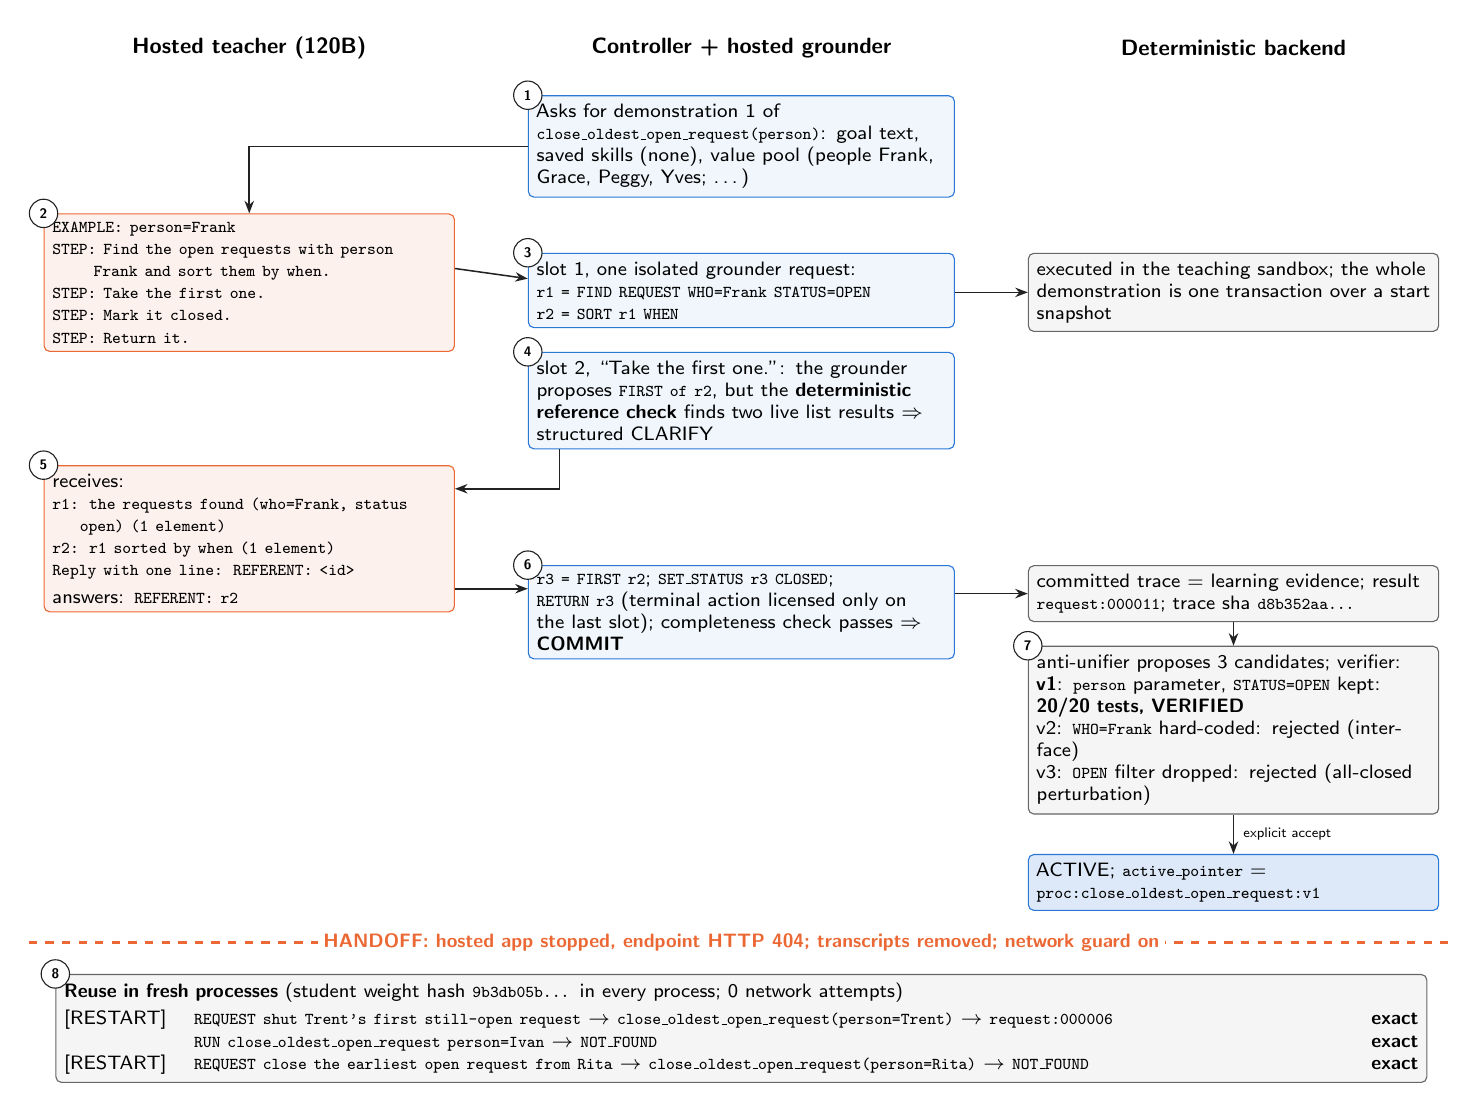
\begin{tikzpicture}[font=\sffamily\scriptsize,
  T/.style={draw=semorange, fill=semorange!9, rounded corners=2pt, text width=50mm, align=left, inner sep=3pt},
  C/.style={draw=semblue, fill=semblue!7, rounded corners=2pt, text width=52mm, align=left, inner sep=3pt},
  B/.style={draw=inkmuted, fill=black!4, rounded corners=2pt, text width=50mm, align=left, inner sep=3pt},
  arr/.style={-{Stealth[length=1.6mm]}, line width=0.55pt, draw=ink},
  num/.style={circle, draw=ink, fill=white, inner sep=0.6pt, font=\sffamily\tiny\bfseries, minimum size=3.6mm},
  hdr/.style={font=\sffamily\footnotesize\bfseries}]
\providecommand{\sq}[1]{{\ttfamily\fontsize{6.4}{7.6}\selectfont #1}}
\def\XT{0} \def\XC{6.25} \def\XB{12.5}
\node[hdr] at (\XT,0.6) {Hosted teacher (120B)};
\node[hdr] at (\XC,0.6) {Controller + hosted grounder};
\node[hdr] at (\XB,0.6) {Deterministic backend};
\node[C, anchor=north] (c1) at (\XC,0) {Asks for demonstration 1 of \sq{close\_oldest\_open\_request(person)}: goal text, saved skills (none), value pool (people Frank, Grace, Peggy, Yves; \dots)};
\node[T, anchor=north] (t1) at ($(c1.south -| \XT,0)+(0,-2mm)$) {\sq{EXAMPLE: person=Frank}\\ \sq{STEP: Find the open requests with person}\\ \sq{\ \ \ \ \ \ Frank and sort them by when.}\\ \sq{STEP: Take the first one.}\\ \sq{STEP: Mark it closed.}\\ \sq{STEP: Return it.}};
\draw[arr] (c1.west) -| (t1.north);
\node[C, anchor=north] (c2) at ($(t1.north -| \XC,0)+(0,-5mm)$) {slot 1, one isolated grounder request:\\ \sq{r1 = FIND REQUEST WHO=Frank STATUS=OPEN}\\ \sq{r2 = SORT r1 WHEN}};
\node[B, anchor=north] (b1) at (c2.north -| \XB,0) {executed in the teaching sandbox; the whole demonstration is one transaction over a start snapshot};
\draw[arr] ($(t1.north east)+(0,-7mm)$) -- ($(c2.west)+(0,1.5mm)$);
\draw[arr] (c2.east |- b1.west) -- (b1.west);
\node[C, anchor=north] (c3) at ($(c2.south)+(0,-3mm)$) {slot 2, ``Take the first one.'': the grounder proposes \sq{FIRST of r2}, but the \textbf{deterministic reference check} finds two live list results $\Rightarrow$ structured CLARIFY};
\node[T, anchor=north] (t2) at ($(c3.south -| \XT,0)+(0,-2mm)$) {receives:\\ \sq{r1: the requests found (who=Frank, status}\\ \sq{\ \ \ \ open) (1 element)}\\ \sq{r2: r1 sorted by when (1 element)}\\ \sq{Reply with one line: REFERENT: <id>}\\[2pt] answers: \sq{REFERENT: r2}};
\draw[arr] ($(c3.south west)+(4mm,0)$) |- ($(t2.north east)+(0,-3mm)$);
\node[C, anchor=north] (c4) at ($(t2.south -| \XC,0)+(0,6mm)$) {\sq{r3 = FIRST r2}; \sq{SET\_STATUS r3 CLOSED};\\ \sq{RETURN r3} (terminal action licensed only on the last slot); completeness check passes $\Rightarrow$ \textbf{COMMIT}};
\draw[arr] ($(t2.south east)+(0,3mm)$) -- (c4.west |- {$(t2.south east)+(0,3mm)$});
\node[B, anchor=north] (b2) at (c4.north -| \XB,0) {committed trace = learning evidence; result \sq{request:000011}; trace sha \sq{d8b352aa\dots}};
\draw[arr] (c4.east |- b2.west) -- (b2.west);
\node[B, anchor=north] (b3) at ($(b2.south)+(0,-3mm)$) {anti-unifier proposes 3 candidates; verifier:\\
 \textbf{v1}: \sq{person} parameter, \sq{STATUS=OPEN} kept: \textbf{20/20 tests, VERIFIED}\\
 v2: \sq{WHO=Frank} hard-coded: rejected (interface)\\
 v3: \sq{OPEN} filter dropped: rejected (all-closed perturbation)};
\draw[arr] (b2) -- (b3);
\node[B, anchor=north, fill=semblue!16, draw=semblue] (b4) at ($(b3.south)+(0,-5mm)$) {ACTIVE; \sq{active\_pointer} = \sq{proc:close\_oldest\_open\_request:v1}};
\draw[arr] (b3) -- node[font=\sffamily\tiny, right]{explicit accept} (b4);
\coordinate (hy) at ($(b4.south)+(0,-4mm)$);
\draw[semorange, dashed, line width=0.8pt] (hy -| -2.8,0) -- (hy -| 15.3,0);
\node[font=\sffamily\scriptsize\bfseries, text=semorange, fill=white, inner sep=2pt] at (hy -| \XC,0) {HANDOFF: hosted app stopped, endpoint HTTP 404; transcripts removed; network guard on};
\node[B, anchor=north, text width=172mm] (r) at ($(hy -| \XC,0)+(0,-4mm)$) {
\textbf{Reuse in fresh processes} (student weight hash \sq{9b3db05b\dots} in every process; 0 network attempts)\\[2pt]
{[RESTART]} \quad \sq{REQUEST shut Trent's first still-open request} $\rightarrow$ \sq{close\_oldest\_open\_request(person=Trent)} $\rightarrow$ \sq{request:000006} \hfill \textbf{exact}\\
\phantom{{[RESTART]}} \quad \sq{RUN close\_oldest\_open\_request person=Ivan} $\rightarrow$ \sq{NOT\_FOUND} \hfill \textbf{exact}\\
{[RESTART]} \quad \sq{REQUEST close the earliest open request from Rita} $\rightarrow$ \sq{close\_oldest\_open\_request(person=Rita)} $\rightarrow$ \sq{NOT\_FOUND} \hfill \textbf{exact}};
\foreach \n/\nd in {1/c1,2/t1,3/c2,4/c3,5/t2,6/c4,7/b3,8/r}{\node[num] at (\nd.north west) {\n};}
\end{tikzpicture}
}
\caption{Worked example \id{dev_a-022-S15}, Arm D. Numbered steps follow the actual event order. The hosted grounder's first reading of ``Take the first one.'' already pointed at \id{r2}; the controller clarified anyway because its deterministic reference rule saw two live list results. The anti-unifier produced three candidates; only v1 survived verification.}
\label{fig:s15}
\end{figure}

The teacher (1{,}285 input and 1{,}129 output tokens for the lesson) wrote a four-step lesson with \texttt{EXAMPLE: person=Frank}. The first line was grounded as a FIND followed by a SORT, producing two list results. For ``Take the first one.'' the controller's reference rule found two live candidates, so it asked a structured question listing \id{r1} (the found requests) and \id{r2} (\id{r1} sorted by when), and the teacher answered \texttt{REFERENT: r2}. The remaining slots grounded directly, RETURN was licensed on the last slot, the completeness check passed, and the demonstration committed with result \id{request:000011}. From this single committed trace the anti-unifier proposed three candidates. The verifier accepted v1 (parameter \id{person}, \id{STATUS=OPEN} kept) with 20 of 20 tests (Table~\ref{tab:verifier}); it rejected v2, which hard-coded \id{WHO=Frank}, at the interface check, and v3, which dropped the \id{OPEN} filter, at the all-closed perturbation. The two registered false-accept probes (frozen value, dropped constant filter) were also rejected. After handoff, three post-restart requests in new wording were served from the library: Trent's request was closed and returned exactly (\id{request:000006}), and the Ivan and Rita requests correctly returned NOT\_FOUND.

\begin{table}[t]
\centering\small
\caption{Verifier tests for the accepted candidate in the worked example.}
\label{tab:verifier}
\resizebox{\linewidth}{!}{\begin{tabular}{lr}
\toprule
Verifier test family & Passed\\
\midrule
static validation & 1/1\\
interface / signature & 1/1\\
source replay & 1/1\\
counterfactual argument substitution & 2/2\\
state perturbation (all closed / alternate closed) & 4/4\\
negative cases (missing input, wrong type, empty result, ambiguous entity, deleted object, empty world) & 6/6\\
rollback injection after each state-changing step & 4/4\\
determinism & 1/1\\
\midrule
Total & 20/20\\
\bottomrule
\end{tabular}
}
\end{table}

\paragraph{Two caveats.} First, Frank had only one open request, so in the demonstration the SORT and the choice of \id{r2} over \id{r1} made no observable difference; the clarification supplied identifying information (the intended referent) that behavioral evidence could not. The program's use of SORT comes from the lesson text, not from anything the trace could have distinguished. Second, only Trent was a positive reuse case; Ivan and Rita returned NOT\_FOUND. Whether the stored procedure picks the oldest of several open requests at reuse time is therefore untested by this example.

\section{Integrity, invalid runs and amendments}\label{sec:integrity}

We list every event that affected the validity or interpretation of a reported run. Full records are in each experiment's engineering log and in Appendix~\ref{app:invalid}.

\begin{itemize}
\item \textbf{TTP attempt 1 was invalid.} The hosted grounder emitted a CHILD action without its required \id{of} field; it passed validation and crashed one Arm D acquisition. Per the registered engineering policy the whole run was archived as invalid, the defect was fixed in general form (a required-field check plus a no-crash guard; Amendment~002), and FINAL\_DEV was rerun from scratch on a freshly seeded DEV set. The archived run's summaries and diagnostic are released.
\item \textbf{TTP Amendment 003.} After TTP's valid run, a controller defect was found: the two-demonstration rule counted demonstration indices rather than committed demonstrations. In one scenario (\id{dev-019-S14L}) an aborted first demonstration left an evaluator-injected legal-bad demonstration to be learned alone, activating one legal-bad procedure in each of Arms A and C. No Arm D target was affected. The A/C safety results of that run are therefore not a valid measurement; the fix was unit-tested, not rerun within TTP, and became RCI's baseline.
\item \textbf{RCI Stage 0C teardown targeted the wrong app.} The ceiling-diagnostic script called the inherited teardown helper without setting its app name; it tried to stop the absent HTG app (return code 1), and the RCI endpoint remained reachable (401). This was repaired immediately by stopping the correct app and verifying 404. Stage 0C was acquisition-only and non-confirmatory; no reuse ran under it.
\item \textbf{The LOCKED 401 race} (Section~\ref{sec:locked}).
\item \textbf{Evaluator-only defects} found after runs and repaired with run data unchanged: in HTG, the judge process lacked credentials (labels regenerated later from saved lessons with a separately verified teardown) and a parameterless-reference scoring bug (one spurious wrong action per arm; the Arm D decision is unchanged either way).
\item \textbf{Superseded development attempts} in PDISC (DEV v1, v2) and PDX (a scenario-design defect; teacher truncation at a 1{,}200-token cap). In PDISC, the first LOCKED set was archived unopened as invalidated-before-run.
\item \textbf{Post-run code edits in the release.} Frozen-file hashes in the released tree match their freeze manifests except four documented post-run edits: TTP \id{teacher/transactional.py} and \id{tests/test_ttp.py} (Amendment~003), HTG \id{evaluator/behavior.py} (the evaluator repair) and RCI \id{htg_evaluate.py} (the post-RCI teardown fix). Path sanitization and one portability edit are recorded file-by-file with original and released hashes.
\end{itemize}

\section{Discussion}\label{sec:discussion}

\paragraph{External memory versus weights.} Placing the learned skill outside the network made three things cheap that are hard in weight space: inspecting exactly what was learned (Figure~\ref{fig:s15}, step 7), rejecting it before it can act, and keeping it through restarts without any interference with the model. The cost is scope: only what the step language can express can be learned, and the model's own competence does not improve.

\paragraph{Query-mediated state versus monolithic context.} The most consequential design choice is not the procedure library but the decision that no model holds state. Monolithic agents scale their memory by scaling context, retrieval or weights, and each of these puts the model in charge of reading and maintaining that state. In \semvm\ the model's job at every step is to translate one bounded input into one typed proposal; persistence, identity, bookkeeping and execution are properties of the runtime. This is what makes the teacher removable: nothing the student needs after handoff lives in a transcript or a context window. It is also a limitation: whatever cannot be expressed as a typed query or program over the world model cannot be used at all.

\paragraph{Verification as learning.} In this system the decision that something has been learned is the verifier's, not the teacher's. That shifts the burden to the evidence. In every recorded case in the lineage where a wrong program was accepted, the evidence itself was wrong, incomplete or vacuous (a lost second demonstration in NL\_TEACH, a mis-grounded empty evidence set in PDX, truncated or unrepaired demonstrations in HTG, a legal-bad demonstration learned alone before TTP's Amendment~003).

\paragraph{Completeness versus consistency.} The HTG failures show that consistency checks are insufficient: a program can be consistent with every committed trace while the traces omit part of the lesson. TTP's move was to make completeness a precondition of evidence admission rather than a property to be inferred later. Since then, every committed Arm D demonstration has been behaviorally exact (TTP, both RCI draws and LOCKED); completeness does not protect against a lesson that is complete but semantically wrong, which is the one wrong committed action in RCI (Arm F).

\paragraph{Interactive clarification.} Clarification is the channel through which a teacher supplies information that behavior cannot. The worked example shows both sides: the structured question elicited the intended referent even though the trace could not distinguish it, but the controller also clarified when the grounder had already chosen correctly. In RCI the hosted recovery teacher resolved 12 of 12 recovery events in Arm E, while replaying registered rephrasings (Arm B) grounded 0 of 14 recovery slots; in TTP, structured reference choice was exact in 2 of 3 events. These are small numbers, but they suggest that the form of the question matters as much as who answers it.

\paragraph{Teacher availability.} The teacher is required to grow the library and not required to use it. That is a real dependency. In the current system, a new skill needs a demonstration from somewhere, and the student cannot generate one for a skill it does not have.

\section{Limitations}\label{sec:limitations}

\begin{itemize}
\item \textbf{Synthetic, bounded domain.} One personal-organizer world, a 21-primitive step language, and curricula drawn from 13--15 procedure families plus composites. Requests at reuse time are controlled paraphrases, not open English.
\item \textbf{Small samples.} Each DEV draw has 36 targets and LOCKED has 23; a perfect LOCKED score is consistent with a system that errs at a few percent per target.
\item \textbf{LOCKED is not a clean pass.} The preregistered teardown-proof condition failed (Section~\ref{sec:locked}).
\item \textbf{Strict structural metric.} Learned-exact requires identity with a reference program; behaviorally equivalent alternatives count as failures, which penalizes some correct teaching and depends on the reference programs chosen.
\item \textbf{Where the language understanding sits.} In the final configuration the hosted 120B model does both teaching and line grounding during acquisition; the frozen 1.5B model's role is post-handoff request interpretation behind deterministic checks. The results say nothing about the 1.5B model's ability to understand lessons.
\item \textbf{Teacher dependence.} Library growth requires a teacher or other source of usable demonstrations.
\item \textbf{One hosted model family.} Teacher, grounder and judge are one frozen checkpoint in separate roles; results may not transfer to other teachers. vLLM at temperature 0 is not bitwise repeatable, so response caches are the experimental record.
\item \textbf{Development reuse.} DEV sets were used for engineering within experiments (notably NL\_TEACH's three iterations), so DEV numbers there are optimistic. RCI used two fresh draws with no change between them.
\item \textbf{Author and scale.} Single-author research with small compute budgets (total hosted spend about \$14.6 across the four hosted experiments); no external replication yet.
\item \textbf{Released blind sets.} The sealed LOCKED sets that were never run (NL\_TEACH, PDX, HTG/TTP) have their contents withheld, but the HTG/TTP sealed sets were generated from the same template file as the RCI LOCKED set, which is released; they should no longer be treated as blind.
\end{itemize}

\section{Future work}\label{sec:future}
These are hypotheses and plans, not results. (1) A clean LOCKED replication on a newly sealed set with the corrected teardown helper. (2) Behavioral rather than structural learned-exact metrics, registered before a new DEV. (3) Richer state diversity in evidence (the S15 caveats suggest requiring multi-element witnesses for SORT/FIRST skills). (4) Other teacher sources: humans, different models, or documentation, which would test whether the protocol rather than this particular teacher carries the result. (5) Larger and less templated domains, and English requests at reuse time. (6) Library scaling: retrieval among hundreds of procedures, versioning when a skill is re-taught, and composition depth beyond one.

\section{Conclusion}\label{sec:conclusion}
A frozen small model plus a deterministic runtime acquired new procedures from a temporary 120B teacher and kept them after the teacher was gone. In the final configuration this happened at \rciDLearnedPooled\ across two independent development draws with no unsafe committed behavior, and at \lockedLearned\ on a sealed test set whose preregistered teardown-proof condition nonetheless failed. The lineage suggests that the hard parts were not execution or retention but the teaching channel, and that treating a demonstration as a transaction and verifying programs against evidence carried most of the weight. What the system learns is narrow, inspectable and permanent; how much it can learn still depends on having someone to learn from.

\section*{Reproducibility and artifact availability}\label{sec:repro}
The repository contains the as-run code of each experiment (not refactored, so that freeze-manifest hashes remain checkable), preregistration documents, locks and manifests, result JSONs, engineering logs, raw teacher, grounder and judge responses keyed by request hash, slot ledgers, teaching transactions, verification records, procedure-store snapshots and handoff and network audits. Reproduction is tiered: (1) fully local unit suites and record replays that need no hosted model (\id{scripts/run_tests.sh}: 127/127 passing at release; \id{scripts/verify_rci_rescore.py}: every RCI metric recomputed from the released per-scenario records, 0 differences in 2{,}530 values); (2) teacher/grounder integration, which requires deploying the same open-weight checkpoint; (3) exact historical results, which are reproduced from the released response caches because temperature-0 serving is not bitwise repeatable. No license file is included; no license has been chosen. See \id{docs/reproduction.md}.

\section*{Use of AI assistance}
Experiment code, analysis scripts and drafts of this paper were written with the help of an AI coding assistant working under the author's direction. All reported numbers are generated by scripts from the released result files.

{\small
\bibliographystyle{plainnat}
\bibliography{references}
}

\appendix
\section{Lineage details}\label{app:lineage}
\begin{table}[h]
\centering\small
\begin{tabularx}{\linewidth}{@{}l>{\raggedright}X>{\raggedright\arraybackslash}X@{}}
\toprule
Experiment (directory) & Arms / suites & Registered outcome, stop rule \\
\midrule
\id{SEMVM_END_TO_END_POC_V1} & FULL, GOLD\_IR; DEV 30, LOCKED 20 & RESULT A; controlled language only (Amendment 001) \\
\id{SEMVM_PROCEDURE_DISCOVERY_POC_V1} & DISCOVERED, GOLD\_PROC; DEV v3 30, LOCKED\_v2 20 & RESULT A; LLM proposal adds nothing over anti-unification \\
\id{SEMVM_NATURAL_LANGUAGE_PROCEDURE_TEACHING_V1} & NL\_TEACH, GOLD\_TRACE, FORMAL\_TEACH; DEV 30 (V1, V1.1, V1.2) & RESULT B + safety stop; LOCKED not run (author ruling) \\
\id{SEMVM_LLM_TO_SEMVM_PROCEDURAL_DISTILLATION_V1} & TEACHER, SCRIPTED, controls; DEV 30 & RESULT E/F conditions; LOCKED not run \\
\id{SEMVM_HOSTED_TEACHER_GROUNDER_V1} & A, B, C, D + controls; DEV 30 & RESULT G + E; LOCKED not run \\
\id{SEMVM_TRANSACTIONAL_TEACHING_PROTOCOL_V1} & A, B, C, D + controls; DEV2 30 (attempt 2) & RESULT D; LOCKED not run \\
\id{SEMVM_RECOVERY_CAPACITY_ISOLATION_V1} & B, E, F, D + controls; DEV-A 30, DEV-B 30; LOCKED 20 (D + controls) & Stage 1 RESULT A pattern; LOCKED behavioral pass, teardown proof failed \\
\bottomrule
\end{tabularx}
\end{table}

\section{Preregistered gates and budgets (RCI)}\label{app:gates}
Arm D pooled gates: learned, scenario and distilled exact $\ge .90$ (minimum counts 65/72, 54/60, 58/64); grounding behavioral exact $\ge .95$ (68/71 given the realized denominator); per-replicate floor .80 on all four. Safety, each replicate: wrong behavioral actions, detectable-bad, legal-bad, conflicting and vacuous activations, verifier false accepts and crashes, incomplete commits, unrequested RETURN and ambiguous references executed all $=0$; demonstration completeness and committed-trace exactness $=1$. Backend: source replay, counterfactual, rollback $=1$; argument binding $\ge .95$; unseen-argument, restart, disconnect and stored reuse given acquisition $=1$; hosted teardown verified $=1$; post-handoff hosted calls and network attempts $=0$; student neural hash invariant. Controls (GOLD\_TRACE, FORMAL\_TEACH) exact. Controller budgets: 2 clarification and 2 rephrase exchanges per slot, 3 demonstrations and 10 teacher turns per target, 8 teacher turns per demonstration, 2 EXAMPLE requests per demonstration. Grounder: reasoning low, 4{,}096 tokens, 1 retry.

\section{Failure taxonomy}\label{app:taxonomy}
Frozen before Stage 0C (\id{spec/FAILURE_TAXONOMY_V1.json}). Layers: provider (truncation, transport, runtime); teacher initial (semantic error, missing content, format); grounder initial (op, argument, relation, reference, sequence, scope); recovery (grounder false clarification, grounder/teacher recovery semantic error, teacher recovery missing content or format, clarification/rephrase/teacher-turn/demonstration budget); controller (state, reference, evidence count, protocol violation); evidence (insufficient variation, unresolved conflict, non-vacuity failure); procedure (abstraction, retrieval, verifier false accept, false reject, crash). The earliest-cause rule walks a target's demonstrations chronologically (skipping registered probe demonstrations), takes the first that did not end committed-and-behaviorally-exact, and within it applies the precedence teacher $\rightarrow$ grounder $\rightarrow$ controller $\rightarrow$ evidence $\rightarrow$ procedure; a provider failure is the cause only if nothing diverged earlier.

\section{Verifier}\label{app:verifier}
Stages 0--6 of \id{procedure/verify.py}: static validation (types, effects, call depth); interface (the candidate's parameters match the declared signature); replay of each source trace; counterfactual substitution of unseen values, compared with the unabstracted trace under the same substitution; state perturbations (e.g.\ all-closed, alternate-closed); negative cases; rollback injection after each state-changing step (the world hash must be unchanged); determinism. The candidate is VERIFIED only if every test passes; activation additionally requires an explicit accept. Registered false-accept probes (frozen value, dropped constant filter, parameterized constant, wrong scope) are run against the same evidence and must be rejected.

\section{Prompts and protocol cards}\label{app:prompts}
The teacher card (sha256 \id{78adbf75...}) and grounder card (sha256 \id{6c11956f...}) are in \id{teacher/protocol.py} and \id{student/hosted_grounder.py}; their hashes are recorded in \id{locks/FINAL_CONFIG_FREEZE.json}. An excerpt of the teacher card:
\begin{Verbatim}
You are a TUTOR. You teach a small assistant (the STUDENT) a new reusable skill. The
student cannot see your reasoning; it only reads the lines you write, executes them
one by one on its personal-organizer database, and learns the skill from what it
successfully executed.
...
TEACH EXACTLY THE REQUESTED SKILL (goal-faithfulness contract)
- Do not add filters, restrictions, state predicates (open / closed), ordering
  criteria, constants, entity scopes or side conditions unless the skill description
  explicitly requires them, or a saved skill's signature makes them necessary.
...
SAVED SKILLS
- To use a saved skill, always write "Call <skill name> with <input> <value>" ...
\end{Verbatim}
The student's structured reference question, verbatim from the worked example:
\begin{Verbatim}
For step 2 ("Take the first one.") more than one earlier result fits:
  r1: the requests found (who=Frank, status open) (1 element), from the step "Find the
      open requests with person Frank and sort them by when."
  r2: r1 sorted by when (1 element), from the step "Find the open requests with
      person Frank and sort them by when."
Reply with one line: REFERENT: <id>
\end{Verbatim}

\section{Examples}\label{app:examples}
The accepted program of the worked example, as stored in \id{procedures.sqlite}:
\begin{Verbatim}
PROCEDURE close_oldest_open_request(person:PERSON)
$v0 = FIND REQUEST WHERE SELF.WHO={person} STATUS=OPEN
$v1 = SORT $v0 WHEN
$v2 = FIRST $v1
SET_STATUS $v2 CLOSED
RETURN $v2
END
\end{Verbatim}
The hosted grounder's raw output for the ambiguous line (both attempts identical):
\begin{Verbatim}
{"status": "PLAN", "steps": [{"bind": "r3", "op": "FIRST", "of": "r2"}]}
\end{Verbatim}
Any scenario and arm can be dumped from the released records, and \id{show_scenario.py} prints a scenario's curriculum, lessons and reuse turns:
\begin{Verbatim}
python scripts/dump_case.py --suite dev_a --scenario <id> --arm D
python scripts/show_scenario.py dev_a/<id> --arm D
\end{Verbatim}

\section{Reproduction}\label{app:repro}
Tier 1 (local, no hosted model): \id{scripts/run_tests.sh} runs 8 suites (127 tests) and writes \id{release_tests/SUMMARY.json}; \id{scripts/verify_rci_rescore.py} recomputes all RCI metrics from records and compares them with the released summaries; \id{scripts/make_figures_tables.py} regenerates every number, table and data figure in this paper from the released JSONs. Tier 2 (integration): deploy gpt-oss-120b (checkpoint sha256 \id{0fc58fd2...}) with vLLM 0.11.0, 32{,}768 context, and point the evaluator at it; new responses will differ from the cached ones. Tier 3 (historical): the evaluators replay from the role-scoped response caches keyed by request hash, which are the experimental record.

\section{Invalid runs and amendments}\label{app:invalid}
\begin{tabularx}{\linewidth}{@{}l>{\raggedright}X>{\raggedright\arraybackslash}X@{}}
\toprule
Event & What happened & Disposition \\
\midrule
E2E Amendment 001 & input-language boundary (controlled language; commands deterministic) & registered before implementation \\
PDISC DEV v1/v2; LOCKED v1 & argument-text failures; one-shot design defect; plan-equivalence tie & general fixes; LOCKED v1 archived unopened; LOCKED\_v2 sealed \\
NL\_TEACH V1, V1.1 & 9 then 2 unsafe executions & Amendments 002, 003; V1.2 final; LOCKED not run \\
PDX DEV attempts 1, 2 & scenario-design defect; 32/98 teacher replies truncated at 1{,}200 tokens & archived; cap 4{,}096; final DEV \\
HTG evaluator defects & judge without credentials; parameterless-reference scoring & evaluator-only rescore; decision unchanged \\
TTP attempt 1 & malformed CHILD crashed an acquisition & archived INVALID; Amendment 002; fresh DEV2 \\
TTP Amendment 003 & committed-evidence count & A/C safety invalid; D unaffected; RCI baseline \\
RCI Stage 0C & teardown targeted wrong app & repaired, 404 verified; acquisition-only \\
RCI LOCKED & handoff probe 401 accepted as destroyed & strict rescore reported; not rerun \\
\bottomrule
\end{tabularx}

\section{Cost}\label{app:cost}
Hosted spend (Modal, H100): PDX \$4.78, HTG \$2.58, TTP \$3.62, RCI \$3.57 (Stage 0C \$0.55; DEV-A, DEV-B and LOCKED about \$1 each); E2E \$0.0011 (CPU equivalence check); PDISC and NL\_TEACH ran locally (RTX 3060 / 2060). In PDX the hosted teacher used 2.2 turns, 1.2 demonstrations and 1.2 student questions per skill on average, about 0.17 exactly verified skills per 1{,}000 teacher tokens. In the worked example the lesson call used 1{,}285 input and 1{,}129 output tokens and the clarification 1{,}427 and 216. Procedure libraries are about 50\,KB per scenario; the student's 1.54B parameters are unchanged throughout.


\section{Project history (background)}\label{app:history}
This appendix summarizes the preregistered experiments that preceded the seven in Section~\ref{sec:lineage}. It is compiled from the author's consolidated project report of 2026-09-21 and, for the last phase, from the individual result reports. \textbf{These experiments' code and results are not included in this release; the numbers below are quoted as reported and are background, not evidence for the paper's claims.} A longer version is \id{docs/project_history.md}.

\begin{center}\small
\begin{tabularx}{\linewidth}{@{}>{\raggedright}p{3.3cm}>{\raggedright}p{4.2cm}>{\raggedright\arraybackslash}X@{}}
\toprule
Phase (dates, 2026) & Question & Reported finding \\
\midrule
1.~Synthetic autoregressive reasoning (Aug 13) & can a small model trade inference compute for parameters via executable derivations? & transition competence $\ne$ execution horizon; a token budget is permission to compute, not a policy \\
2.~External associative memory (Aug 27--30) & can knowledge live in a memory beside a small Transformer? & concepts externalize as readable memory; part of the early gain was lexical binding \\
3.~Control/optimization ladder V6--V12 (Aug 31) & why does in-episode derivation fail? & attention supervision saturated without execution gains; the ceiling was undertraining (seed-variable) \\
4.~Macro-core, ml\_next, neural instructions (Sep 6--7) & where do real-benchmark traces fail? & GSM8K free 0.376 vs oracle state 0.990: state carry dominates; knowledge scales with memory bytes \\
5.~Semantic front-end on GSM8K (Sep 9--10) & map language to a frozen operator set & operator selection plateaued near 0.56; grounding real text is the frontier \\
6.~Synthetic stateful VM v0--v4C.3 (Sep 11--12) & can a small controller act over explicit durable state? & store scaled 1K$\rightarrow$1M records at a constant 32-record working set, final state 1.000 (3 seeds, delexicalized; v2); typed query + typed matching + deterministic projection: relational answers 0.00$\rightarrow$1.00 (v4B.1); 64-turn closed loop at $\sim$24 context tokens vs a 1{,}306-token transcript (v4C) \\
7.~Human language + Wikidata (Sep 12--13) & external knowledge behind a linker & 300 facts taught after freezing survived restart at 1.0 with zero optimizer steps; predicate grounding 0.20 \\
8.~Frozen code LLMs on SWE-bench (Sep 13--15) & can frozen 0.5B--3B models revise from evidence? & no, at any size; polarity not legible from bounded strings \\
9.~Runtime predicates, real code (Sep 15--16) & can a controller know when it is done? & runtime progress predicates: depth 5--12 episode success 0.063 (0.190 with semantic queries) $\rightarrow$ 1.0 \\
10.~Semantic compilation v6E (Sep 16--17) & compile language to composable records & identity and semantics separable; composition stayed at 0 \\
11.~Latent parsers (Sep 17--21) & learn typed records over frozen Qwen features & toy solved (64/64 withheld); real prose fits (811/844) but does not transfer (withheld 0/59) \\
12a.~Typed Qwen frontend (Sep 22--23) & read typed fields from frozen Qwen-0.5B & mid-layer readout 56--58/96 on fresh language; envelope fixed deterministically; no training-side invariance gain \\
12b.~Query-mediated world state (Sep 23--24) & can a frozen backbone + 3.24M head read/write an external store via typed queries? & 0.985 exact; 512-entity store at 29.2 tokens/turn; held-out phrasing 0.367 $\rightarrow$ 0.82 with phrasing diversity (one/two seeds) \\
12c.~MTOP and attachment (Sep 24) & compositional human language & tree exact 0.696 vs 0.512; novel combinations 0.167; novel attachment stuck near 0.80 under LoRA and data fixes \\
12d.~Typed composition (Sep 24--25) & local types, supertags, latent composition & oracle structure assembles exactly; learned predictors fail fit gates; latent factorization collapses \\
12e.~Multi-relation binding (Sep 25--26) & coindexation parent binding & fit failure partly an early-stopping plateau artifact; P0 replay preserves binding (A-005, one seed) $\rightarrow$ the E2E binder \\
\bottomrule
\end{tabularx}
\end{center}

\end{document}
